\documentclass[12pt,letterpaper]{article}
\usepackage[utf8]{inputenc}
\usepackage[spanish,es-tabla]{babel}
\usepackage{graphicx}
\usepackage{xcolor}
\usepackage{geometry}
\usepackage{array}
\usepackage{booktabs}
\usepackage{multirow}
\usepackage{threeparttable}
\usepackage{caption}
\usepackage{float}
\usepackage{tabularx}
\usepackage{parskip}
\usepackage{amsmath}
\usepackage{amssymb}

\captionsetup[table]{font=small}

% --- PAQUETE PARA ENCABEZADOS ---
\usepackage{fancyhdr} 

\captionsetup[table]{font=small}

\geometry{
	letterpaper,
	top=3.5cm, % Aumentamos el margen superior para que quepan lo\textbf{}s logos
	bottom=2.5cm,
	left=2.5cm,
	right=2.5cm,
	headheight=2cm % Espacio para el encabezado
}

% --- CONFIGURACIÓN DEL ENCABEZADO (LOGOS) ---
\pagestyle{fancy}
\fancyhf{} % Limpia encabezado y pie de página
\fancyhead[L]{
\includegraphics[height=1.0cm]{logos/mag_ciencia_datos_innovación_color.png}} % Ajusta el nombre de tu archivo
\fancyhead[R]{
\includegraphics[height=1.0cm]{logos/Logo CDIA 2024-01-01.png}} % Ajusta el nombre de tu archivo
\renewcommand{\headrulewidth}{0pt} % Elimina la línea horizontal si no la deseas
\fancyfoot[C]{\thepage} % Número de página al centro

\begin{document}
	
	% ==========================================
	
	% FORMATO DE TABLAS (autoexplicativas)
	
	% ==========================================
	
	\newcommand{\tablaauto}[4]{%
		\begin{table}[H]
			\centering
			\captionsetup{font=small}
			\begin{threeparttable}
				\caption{#1}
				\label{#2}
				\small
				\setlength{\tabcolsep}{6pt}
				\renewcommand{\arraystretch}{1.15}
				#3
				\begin{tablenotes}[flushleft]
					\footnotesize
					\item \textit{Nota:} #4
				\end{tablenotes}
			\end{threeparttable}
		\end{table}%
	}
	
	% ==========================================
	% PORTADA
	% ==========================================
	\begin{titlepage}
		\thispagestyle{empty} % Asegura que no haya encabezados aquí
		\centering
		
		% Escudo centrado arriba
		
\includegraphics[height=4cm]{logos/escudo.jpg} \\[0.5cm] 
		
		{\Large \textbf{UNIVERSIDAD DE CONCEPCIÓN}}\\[0.3cm]
		{\Large \textbf{FACULTAD DE INGENIERÍA}}\\[1.5cm]
		
		\vspace{1cm} % Espacio reducido para asegurar que todo quepa
		
		% Título
		{\LARGE \textbf{Estimación de Variables Geometalúrgicas con Machine Learning}}\\[2.5cm]
		
		% Autor
		{\large Por}\\[0.3cm]
		{\large \textbf{Ignacio Enrique Rojas Rodríguez}}\\[2.5cm]
		
		% Descripción (usamos un parbox para controlar el ancho si es necesario)
		\noindent\begin{minipage}{0.85\textwidth}
			\centering
			Tesina presentada a la Facultad de Ingeniería de la Universidad de Concepción para optar al grado de Magíster en Ciencia de Datos para la Innovación
		\end{minipage}
		
		\vspace{1.5cm}
		
		% Profesores
		{\large Profesor guía: Pedro Pinacho}\\[0.2cm]
		{\large Profesor co-guía: José Ulloa}
		
		\vfill % Empuja lo que sigue al final de la página
		
		% Fecha y lugar
		{\large Marzo de 2026}\\
		{\large Concepción, Chile}
	\end{titlepage}
	
	% ==========================================
	% ESTRUCTURA DE ÍNDICES
	% ==========================================
	\pagenumbering{arabic} % Numeración romana para índices
	\tableofcontents
	\newpage
	\listoffigures
	\newpage
	\listoftables
	\newpage
	
	% ==========================================
	% ESTRUCTURA DEL DOCUMENTO
	% ==========================================
	
\section{Introducción}

	La minería contemporánea se encuentra inmersa en un proceso de transformación 
	digital donde la integración de la información es fundamental para asegurar la 
	viabilidad y rentabilidad de los proyectos a largo plazo \cite{Nwaila2024}. En este contexto, la 
	geometalurgia ha emergido como una disciplina crítica que busca vincular las 
	características geológicas de un yacimiento con su respuesta en los procesos 
	de extracción y beneficio metalúrgico \cite{Moreira2021}. Sin embargo, la industria enfrenta un 
	obstáculo estructural en la modelación de estas variables: la profunda asimetría 
	en la densidad de los datos. Mientras que la información geológica tradicional 
	suele ser abundante gracias a extensas campañas de sondaje, los datos 
	geometalúrgicos, tales como la recuperación en peso, son comparativamente 
	escasos debido al alto costo y tiempo que demandan los ensayos de laboratorio \cite{Jia2018}. 
	La recuperación en peso se define como la razón entre la masa del concentrado 
	obtenido y la masa total del mineral alimentado al proceso, expresada 
	matemáticamente como:
	
	\begin{equation}
		R_p (\%) = \left( \frac{Masa_{Conc}}{Masa_{Alim}} \right) \times 100
	\end{equation}
	
	donde $R_p$ es la recuperación en peso, $Masa_{Conc}$ la masa del concentrado 
	final obtenido del circuito y $Masa_{Alim}$ la masa de alimentación al circuito.
	
	Tradicionalmente, la estimación espacial de estas variables se ha abordado 
	mediante herramientas geoestadísticas clásicas \cite{Garnier2022}. Si bien estos métodos son 
	robustos en escenarios de alta densidad de muestreo, su aplicación sobre 
	conjuntos de datos reducidos resulta en un proceso lento, iterativo y altamente 
	dependiente del juicio experto para forzar supuestos de estacionariedad \cite{Emery2007} o anisotropía \cite{Mery2024}. Además, estos flujos de trabajo están fuertemente condicionados 
	por el uso de licencias de software propietario de alto costo, lo que limita 
	la capacidad de las empresas para experimentar y democratizar el análisis de 
	sus propios datos \cite{Nwaila2024}.
	
	Frente a esta problemática, la presente tesina, desarrollada en el marco del 
	Magíster en Ciencia de Datos para la Innovación de la Universidad de Concepción, 
	propone incorporar Machine Learning para la estimación de variables 
	geometalúrgicas \cite{Nwaila2024}. El objetivo central es construir un Producto Mínimo Viable 
	(MVP) programado en Python que automatice la estimación espacial de la 
	recuperación en peso a partir de un conjunto reducido de datos \cite{Moreira2021}. La hipótesis 
	subyacente es que los algoritmos de aprendizaje automático, tanto no supervisados 
	para la definición de dominios como supervisados para la estimación continua, 
	poseen la flexibilidad matemática necesaria para capturar las complejas 
	relaciones espaciales del mineral sin depender de las rígidas restricciones 
	paramétricas de la geoestadística tradicional \cite{Moreira2021}.
	
	Para demostrar la validez de esta propuesta, el documento se estructura 
	siguiendo el ciclo de vida de un proyecto de ciencia de datos aplicado a la 
	minería. En primer lugar, se expone el marco y alcance de la propuesta, 
	definiendo el problema de negocio y los objetivos del MVP. A continuación, 
	se detalla el proceso de obtención, depuración y transformación estadística 
	de la base de datos geometalúrgica. Posteriormente, se presenta un análisis 
	exploratorio espacial que justifica la elección de las variables predictoras. 
	El núcleo de la investigación se desarrolla en la sección de modelado, donde 
	se implementan técnicas de agrupamiento tridimensional y se contrastan modelos 
	predictivos avanzados contra el modelo de bloques vigente de la empresa. 
	Finalmente, se interpretan los resultados desde una perspectiva técnica y 
	operacional, concluyendo con los hallazgos y el impacto potencial de incorporar 
	este flujo de trabajo en la industria minera.
		
	\section{Presentación de la propuesta}
	
	La presente propuesta consiste en desarrollar e implementar una alternativa 
	metodológica para la estimación de variables geometalúrgicas, integrando 
	técnicas de ciencia de datos y aprendizaje automático (Machine Learning) al 
	flujo de trabajo tradicional de la industria minera. Mediante la construcción 
	de un Producto Mínimo Viable (MVP) programado íntegramente en Python, se busca 
	comparar los resultados de esta nueva aproximación con las estimaciones 
	convencionales, evaluando la viabilidad de la propuesta en términos de 
	precisión técnica, reducción de tiempos de procesamiento y disminución de la 
	dependencia de software comercial de alto costo.
		
	\subsection{Problema}
	
	La industria minera enfrenta el desafío constante de integrar información 
	geológica y geometalúrgica para sustentar la planificación de largo plazo. 
	Sin embargo, existe una profunda asimetría en la densidad de la información: 
	mientras los datos geológicos (como litología o alteración) suelen ser 
	abundantes, los datos propiamente geometalúrgicos son comparativamente escasos. 
	Variables críticas como la recuperación en peso requieren ensayos de laboratorio 
	de alto costo, lo que limita su cantidad a unos pocos cientos de registros 
	dentro de un yacimiento. Esta escasez de datos genera una dificultad para la 
	estimación espacial continua.
	
	Los enfoques geoestadísticos tradicionales, como el \textit{Kriging}, fueron 
	desarrollados para operar sobre conjuntos de datos suficientemente densos que 
	permitan un estudio variográfico robusto. Aplicar estas metodologías 
	tradicionales a bases de datos reducidas requiere un trabajo experto intensivo 
	para forzar supuestos de estacionariedad, definir elipses de búsqueda y modelar 
	el comportamiento isotrópico o anisotrópico. Como resultado, las estimaciones 
	pueden volverse inestables o excesivamente suavizadas, disminuyendo la confianza 
	en los modelos utilizados para la toma de decisiones. Una estimación poco 
	representativa de la recuperación geometalúrgica impacta directamente en la 
	proyección de tonelajes, el diseño del proceso y los indicadores económicos del 
	proyecto.
	
	Adicionalmente, estos flujos de trabajo dependen fuertemente de licencias de 
	software especializado de alto costo y de rutinas intensivas en tiempo humano. 
	Frente a este escenario, surge la necesidad de explorar si algoritmos de 
	aprendizaje automático, capaces de encontrar relaciones espaciales complejas y 
	no lineales sin requerir los estrictos supuestos paramétricos de la 
	geoestadística, pueden ofrecer estimaciones de calidad comparable o superior, 
	agilizando el proceso y democratizando el uso de los datos mediante lenguajes 
	de programación de código abierto.
	
	\subsection{Acercamiento, actores, dimensiones}
	
	La iniciativa surge del interés por incorporar prácticas de ciencia de datos 
	a la estimación de recursos. El acercamiento metodológico se estructura en un 
	flujo de trabajo ágil y reproducible. En lugar de realizar extensos estudios 
	variográficos, se utilizan técnicas de aprendizaje no supervisado para definir 
	dominios con coherencia espacial y metalúrgica, seguidas de modelos supervisados 
	que aprenden de manera autónoma las relaciones espaciales subyacentes de la 
	variable a estimar.
	
	Los actores principales y beneficiarios directos de esta propuesta son los 
	geólogos, geometalurgistas y planificadores mineros responsables de los 
	proyectos de estimación. A nivel corporativo, el proyecto dialoga con la 
	necesidad estratégica de la empresa de optimizar recursos y explorar 
	alternativas tecnológicas eficientes.
	
	La propuesta abarca tres dimensiones clave:
	\begin{itemize}
		\item \textbf{Dimensión técnica:} Demostrar empíricamente que algoritmos 
		como K-Means y KNN pueden capturar la continuidad y anisotropía espacial 
		de variables escasas con métricas de error competitivas.
		\item \textbf{Dimensión de negocio:} Proveer una alternativa que reduzca 
		los tiempos de modelamiento experto y evalúe la factibilidad de independizar 
		parte del proceso de las costosas licencias de software propietario.
		\item \textbf{Dimensión de adopción tecnológica:} Entregar un MVP en Python 
		que funcione como código base replicable, fomentando la cultura de 
		\textit{Data Science} dentro de los equipos técnicos de la compañía.
	\end{itemize}
	
\subsection{Descripción de la propuesta}

	La propuesta se materializa en un flujo de trabajo computacional (pipeline) 
	focalizado en una variable geometalúrgica crítica y escasamente muestreada: 
	la recuperación en peso. A partir de una base de datos de 1.219 registros de 
	laboratorio, el MVP se encarga de procesar, transformar y modelar la 
	información de principio a fin en un entorno Python.
	
	El proceso inicia con una fase de limpieza y transformación de datos, 
	aplicando una transformación gaussiana (\textit{Normal Score Transformation}) 
	para estabilizar la distribución de la variable objetivo. Posteriormente, se 
	aplica un agrupamiento tridimensional automatizado mediante K-Means, que 
	reemplaza la definición manual de dominios metalúrgicos por una segmentación 
	objetiva basada en la posición espacial y la respuesta metalúrgica de los 
	datos. Con los dominios identificados, se entrenan cuatro modelos predictivos 
	sobre el total de los datos disponibles: K-vecinos más cercanos (KNN), Random 
	Forest, Gradient Boosting y XGBoost, utilizando las coordenadas tridimensionales 
	como variables predictoras.
	
	La validación de los modelos se realizó de forma externa, comparando las 
	predicciones de cada modelo contra los valores reales en los puntos del modelo 
	de bloques vigente de la empresa, estimado mediante Kriging. Esto permite medir 
	de forma objetiva el desempeño del Machine Learning frente al método tradicional, 
	bajo exactamente las mismas condiciones y sobre los mismos puntos de referencia.
	
	\subsection{Descripción del MVP y objetivos}
	
	El producto mínimo viable (MVP) corresponde a un conjunto de \textit{notebooks} y \textit{scripts} en Python que ejecutan secuencialmente la carga de datos, el análisis exploratorio (EDA), el \textit{domaining} no supervisado, el entrenamiento de modelos supervisados y la generación masiva de estimaciones sobre una grilla espacial o "modelo de bloques" sintético, incluyendo sus respectivas métricas de error visuales y numéricas.
	
	\textbf{Objetivo general:}
	Desarrollar y evaluar un flujo de trabajo basado en aprendizaje automático para la estimación espacial de variables geometalúrgicas con datos escasos, contrastando su rendimiento, agilidad y costo de implementación frente a las metodologías geoestadísticas tradicionales utilizadas por la empresa.
	
	\textbf{Objetivos específicos:}
	\begin{itemize}
		\item Diseñar un flujo automatizado para el preprocesamiento y transformación estadística de datos geometalúrgicos.
		\item Implementar técnicas de aprendizaje no supervisado para la delimitación matemática de dominios geometalúrgicos espaciales.
		\item Entrenar y optimizar modelos de aprendizaje supervisado para predecir la 
		recuperación en peso, evaluando su desempeño sobre los puntos de validación 
		del modelo de bloques de la empresa y verificando la coherencia espacial de 
		las estimaciones.
		\item Comparar el desempeño cuantitativo, la coherencia espacial y el esfuerzo operativo del modelo de \textit{Machine Learning} frente al modelo oficial de la empresa.
	\end{itemize}
	
	\subsection{Descripción de validación}
	
	Validar un modelo de estimación espacial presenta un desafío inherente a este tipo de problemas: los puntos no muestreados del yacimiento no tienen un valor de referencia conocido. Para abordarlo, la validación de esta tesina se apoya en tres enfoques complementarios.
	
	El primero es una \textbf{validación estadística interna}. Los modelos se entrenaron con el $100\%$ de los datos disponibles, decisión justificada por el volumen reducido de la base de datos, y su comportamiento se evaluó mediante métricas estándar como el coeficiente de determinación ($R^2$) y la raíz del error cuadrático medio (RMSE). Esto permite medir qué tan bien ajusta el modelo a los datos con los que fue construido.
	
	El segundo es una \textbf{validación geoespacial}. Se verificó que las estimaciones masivas preserven la distribución estadística original y que no introduzcan sesgos sistemáticos en ninguna dirección del espacio. Para esto se analizó la deriva espacial (\textit{drift}) en los ejes Este, Norte y Cota, comprobando que el modelo respeta las tendencias macroscópicas del yacimiento.
	
	El tercero, y más relevante para evaluar el desempeño real del MVP, es una 
	\textbf{validación externa contra el modelo de la empresa}. La compañía cuenta con un modelo de bloques de aproximadamente 380.000 puntos, estimados mediante Kriging utilizando la misma base de datos de laboratorio que se emplea en este trabajo. Para realizar la comparación, se identificó el punto del modelo de la empresa más cercano a cada una de las muestras originales. La distancia promedio entre pares fue de aproximadamente 7 metros, lo que es suficientemente pequeño para asumir que ambos valores, el real de laboratorio y el estimado por Kriging, deberían ser similares. Bajo esa premisa, el Kriging de la empresa actúa como \textit{benchmark}: se midió primero cuánto explica el Kriging de la variabilidad de los datos reales ($R^2 \approx 80\%$), y luego se comparó ese resultado con el desempeño de los modelos de Machine Learning sobre los mismos puntos.
	
	\section{Obtención de datos}
	
	Los datos utilizados en esta investigación provienen de dos fuentes distintas. 
	Por acuerdos de confidencialidad, no se detallan los nombres específicos del 
	yacimiento ni las fechas de las campañas de exploración.
	
	La primera fuente corresponde a una base de datos de sondajes y pruebas 
	geometalúrgicas de laboratorio, provista por una empresa minera externa. La 
	información fue entregada en formato tabular, consolidando en una única estructura 
	la ubicación espacial de las muestras y su respuesta metalúrgica. Esta base contiene 
	$1.219$ registros finales, donde cada uno incluye las coordenadas espaciales 
	tridimensionales (Este, Norte y Cota), junto con la recuperación en peso ($\%$) como 
	variable objetivo principal. Estos registros constituyen la base sobre la cual se 
	desarrolla el análisis exploratorio, la definición de dominios y el entrenamiento 
	de los modelos predictivos.
	
	La segunda fuente es el modelo de bloques vigente de la empresa consultora donde 
	se desarrolla esta tesina, que contiene $343.732$ puntos estimados mediante Kriging. 
	Este modelo fue construido utilizando la misma base de datos de laboratorio, y cubre 
	de forma continua el volumen del yacimiento. Su rol en esta tesina es exclusivamente 
	el de referencia para la validación externa: permite comparar directamente las 
	estimaciones del Machine Learning contra las del método geoestadístico oficial sobre 
	los mismos sectores del yacimiento.
	
	\section{Depuración de datos}
	
	Antes de comenzar con el análisis, se revisó y limpió la base de datos para 
	asegurar que la información que alimenta los modelos sea consistente y confiable.
	
	El conjunto inicial contaba con 1.466 registros. Durante la revisión se identificaron 230 registros con el valor $-99$, que es la convención utilizada en estas bases de datos para indicar que una prueba de laboratorio no tiene resultado. Estos registros fueron eliminados por no aportar información útil para el modelado.
	
	Adicionalmente, se eliminaron 17 registros cuya coordenada Norte superaba los 
	27.000 metros, ya que corresponden a muestras ubicadas fuera del área de interés del yacimiento y podrían introducir ruido en las estimaciones espaciales.
	
	Tras ambos filtros, la base de datos quedó conformada por 1.219 registros válidos, lo que representa el 83,2\% del total original. Este es el conjunto que se utiliza en todas las etapas posteriores del trabajo.
	
	Una vez depurada la base, se analizó la distribución de la variable objetivo. La recuperación en peso presenta una distribución asimétrica, con una cola extendida hacia valores altos, lo que puede afectar el comportamiento de los modelos. Para corregir esto, se aplicó una transformación gaussiana (\textit{Normal Score Transformation}), que ajusta la distribución original hacia una normal estándar con media $\mu = 0$ y desviación estándar $\sigma = 1$. Todas las etapas de modelado se realizaron sobre esta variable transformada.
	
\section{Exploración de datos}

Para entender cómo se distribuyen los datos en el espacio, se generaron 
visualizaciones en tres y dos dimensiones, donde el eje Este corresponde a la 
dirección X, el Norte a la dirección Y y la Cota a la dirección Z. La Figura 
\ref{fig:3d} muestra que la gran mayoría de las muestras presenta valores de 
recuperación inferiores al 21\% (tonos azules), mientras que los valores más altos 
aparecen de forma localizada, lo que sugiere continuidad espacial y no una 
distribución aleatoria.

La Tabla \ref{tab:descriptivos} resume los principales estadísticos descriptivos 
del conjunto de datos.

\begin{table}[h]
	\centering
	\caption{Estadísticos descriptivos de las variables principales.}
	\begin{tabular}{lcccccc}
		\hline
		\textbf{Variable} & \textbf{N} & \textbf{Promedio} & \textbf{Desv. Est.} & 
		\textbf{Mín.} & \textbf{Máx.} \\
		& (1) & (2) & (3) & (4) & (5) \\
		\hline
		Este (m)                  & 1.219 & 9.009,09  & 162,44 & 8.438,38  & 9.381,41  \\
		Norte (m)                 & 1.219 & 24.797,32 & 703,99 & 23.604,57 & 26.790,97 \\
		Cota (m)                  & 1.219 & 2.058,27  & 170,73 & 1.219,74  & 2.312,77  \\
		Recuperación en peso (\%) & 1.219 & 18,00     & 6,63   & 4,35      & 60,87     \\
		\hline
	\end{tabular}
	\begin{flushleft}
		\small \textit{Nota:} Elaboración propia en base a los datos del estudio. 
		(1) = tamaño de muestra, (2) = promedio, (3) = desviación estándar, 
		(4) = mínimo valor observado, (5) = máximo valor observado.
	\end{flushleft}
	\label{tab:descriptivos}
\end{table}

La recuperación en peso tiene una media de 18\% y una mediana de 16,6\%, lo que 
ya sugiere una distribución asimétrica hacia la derecha. Esto se confirma en la 
Figura \ref{fig:hist}, donde el histograma original muestra una cola extendida 
hacia valores altos, con un máximo de 60,87\% que se aleja considerablemente del 
tercer cuartil. Tras aplicar la transformación gaussiana, la distribución adopta 
una forma de campana simétrica, lo que se valida adicionalmente en el gráfico Q-Q 
de la Figura \ref{fig:qq}, donde los puntos se alinean sobre la diagonal de 
referencia.

\begin{figure}[H]
	\centering
	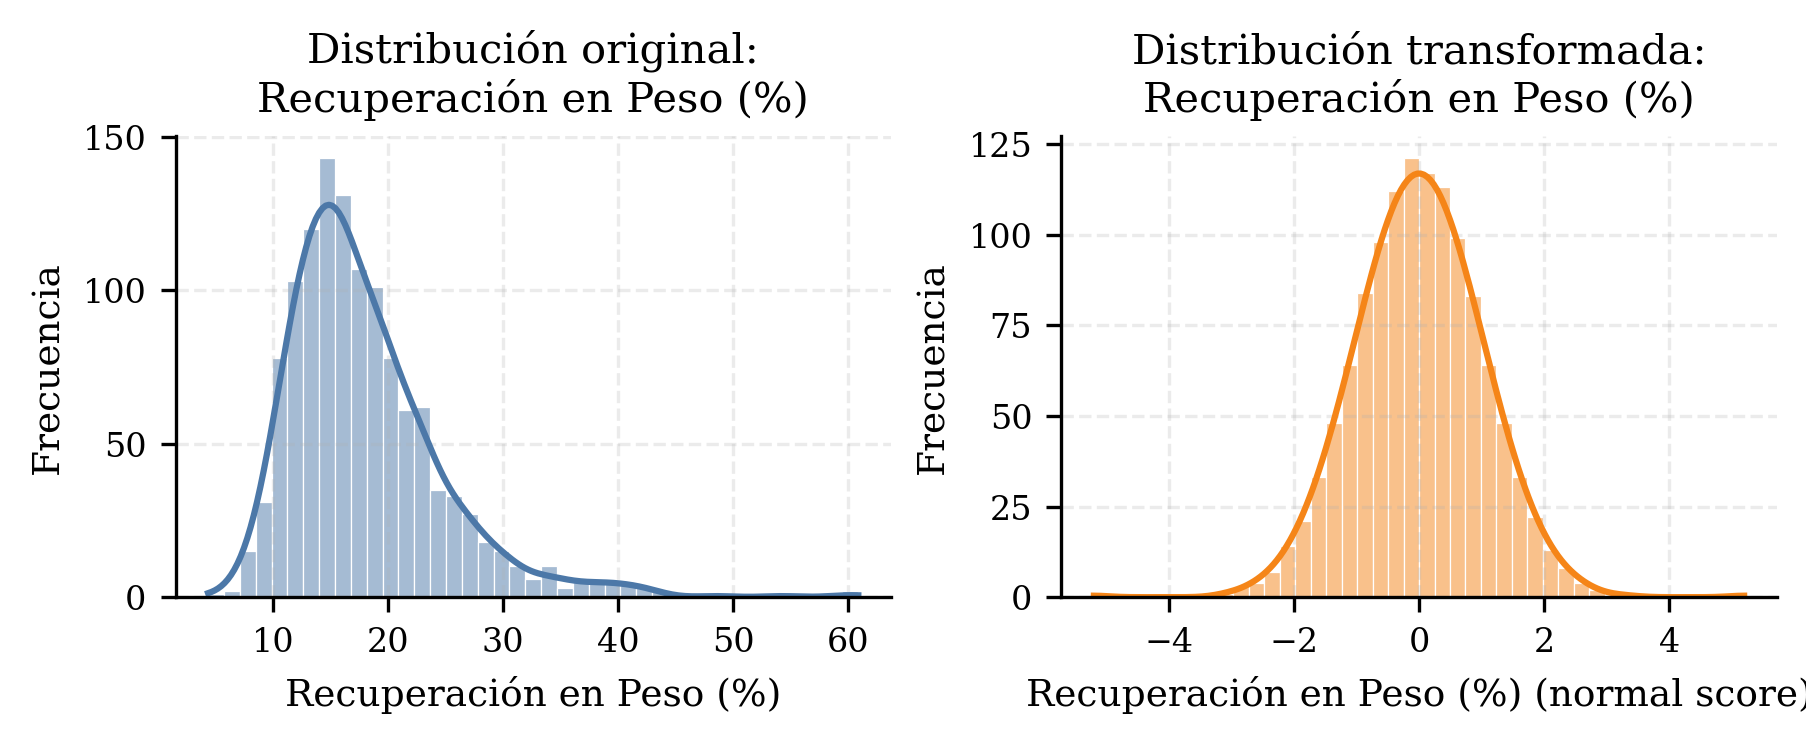
\includegraphics[width=0.8\textwidth]{img_eda/hist_original_vs_gauss_recpe.png}
	\caption{Distribución original y transformada (Normal Score) de la 
		recuperación en peso.}
	\label{fig:hist}
\end{figure}

\begin{figure}[H]
	\centering
	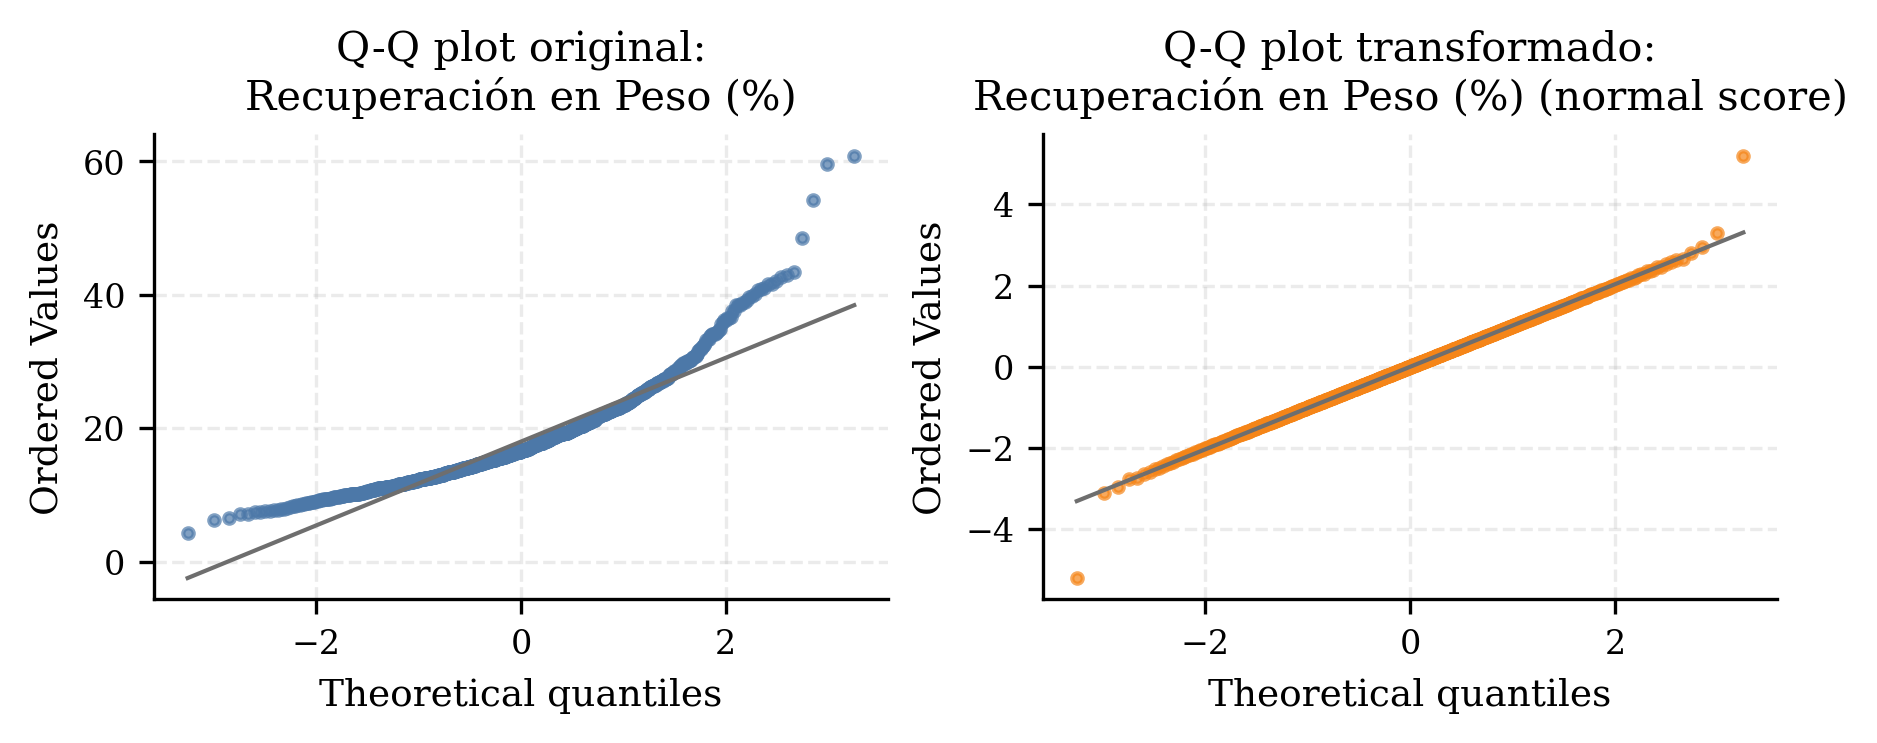
\includegraphics[width=0.8\textwidth]{img_eda/qq_original_vs_gauss_recpe.png}
	\caption{Gráfico Q-Q de la recuperación en peso original y transformada.}
	\label{fig:qq}
\end{figure}

Para entender cómo se distribuyen los datos en el espacio, se generaron 
visualizaciones en tres y dos dimensiones. La Figura \ref{fig:3d} muestra que la 
gran mayoría de las muestras presenta valores de recuperación inferiores al 21\% 
(tonos azules), mientras que los valores más altos aparecen de forma localizada, 
lo que sugiere continuidad espacial y no una distribución aleatoria.

\begin{figure}[H]
	\centering
	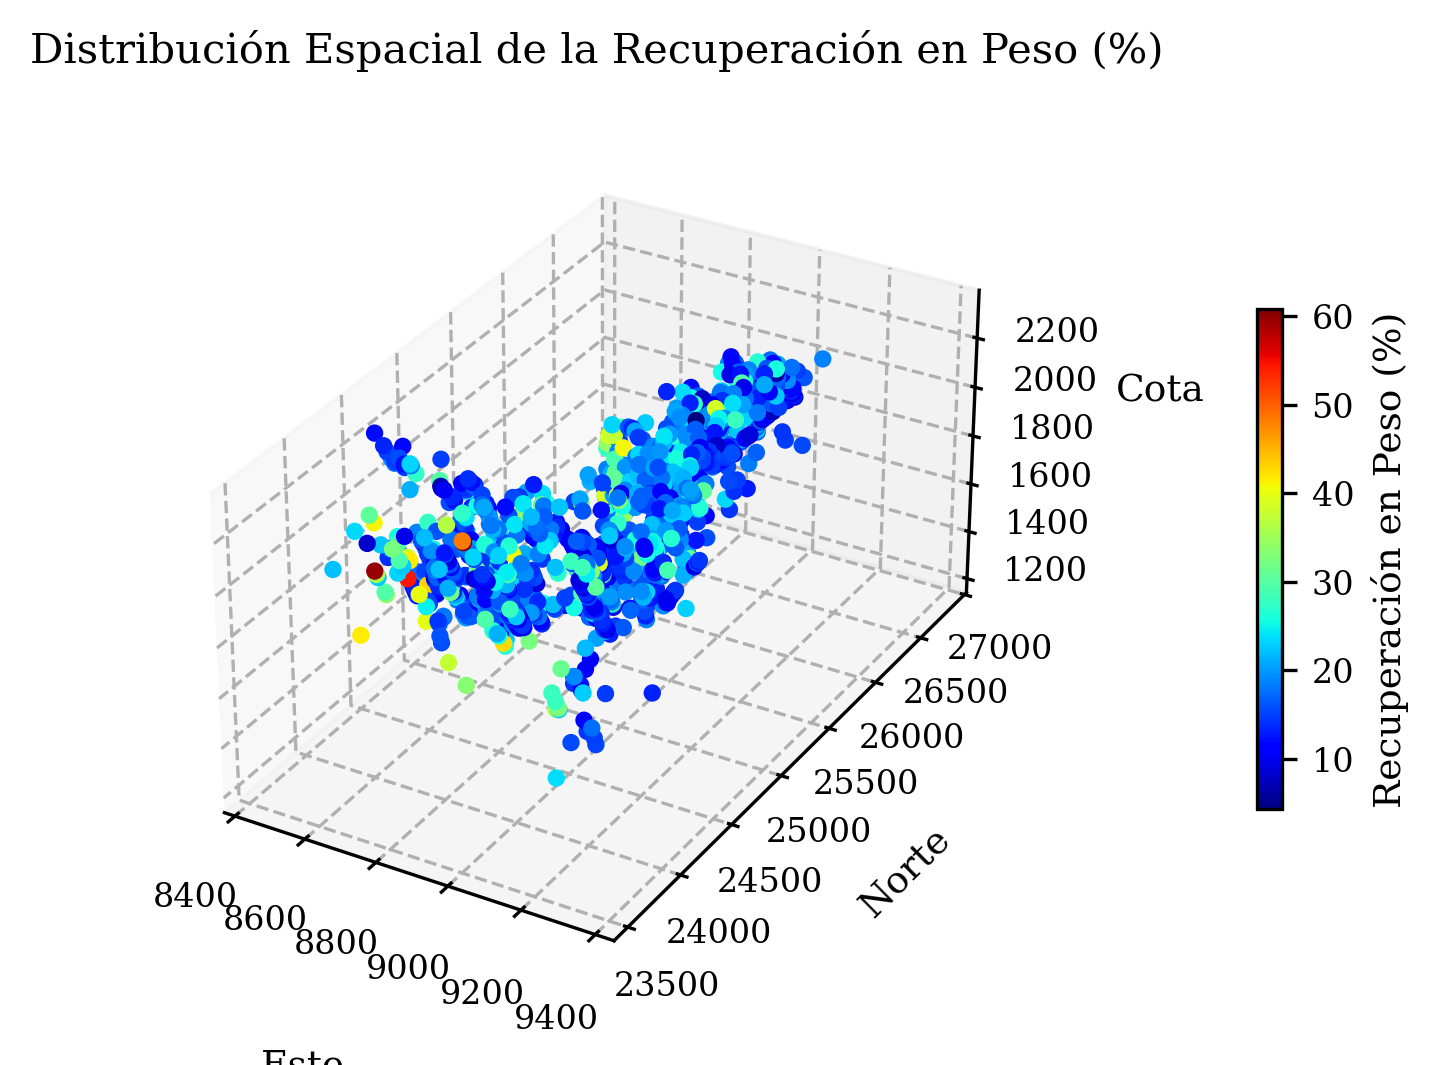
\includegraphics[width=0.8\textwidth]{img_eda/mapa_3d_recpe.png}
	\caption{Distribución espacial 3D de la recuperación en peso.}
	\label{fig:3d}
\end{figure}

Las proyecciones en dos dimensiones de la Figura \ref{fig:2d} permiten identificar 
con mayor claridad la concentración de muestras y la ubicación de las zonas de 
mayor recuperación en cada plano del yacimiento.

\begin{figure}[H]
	\centering
	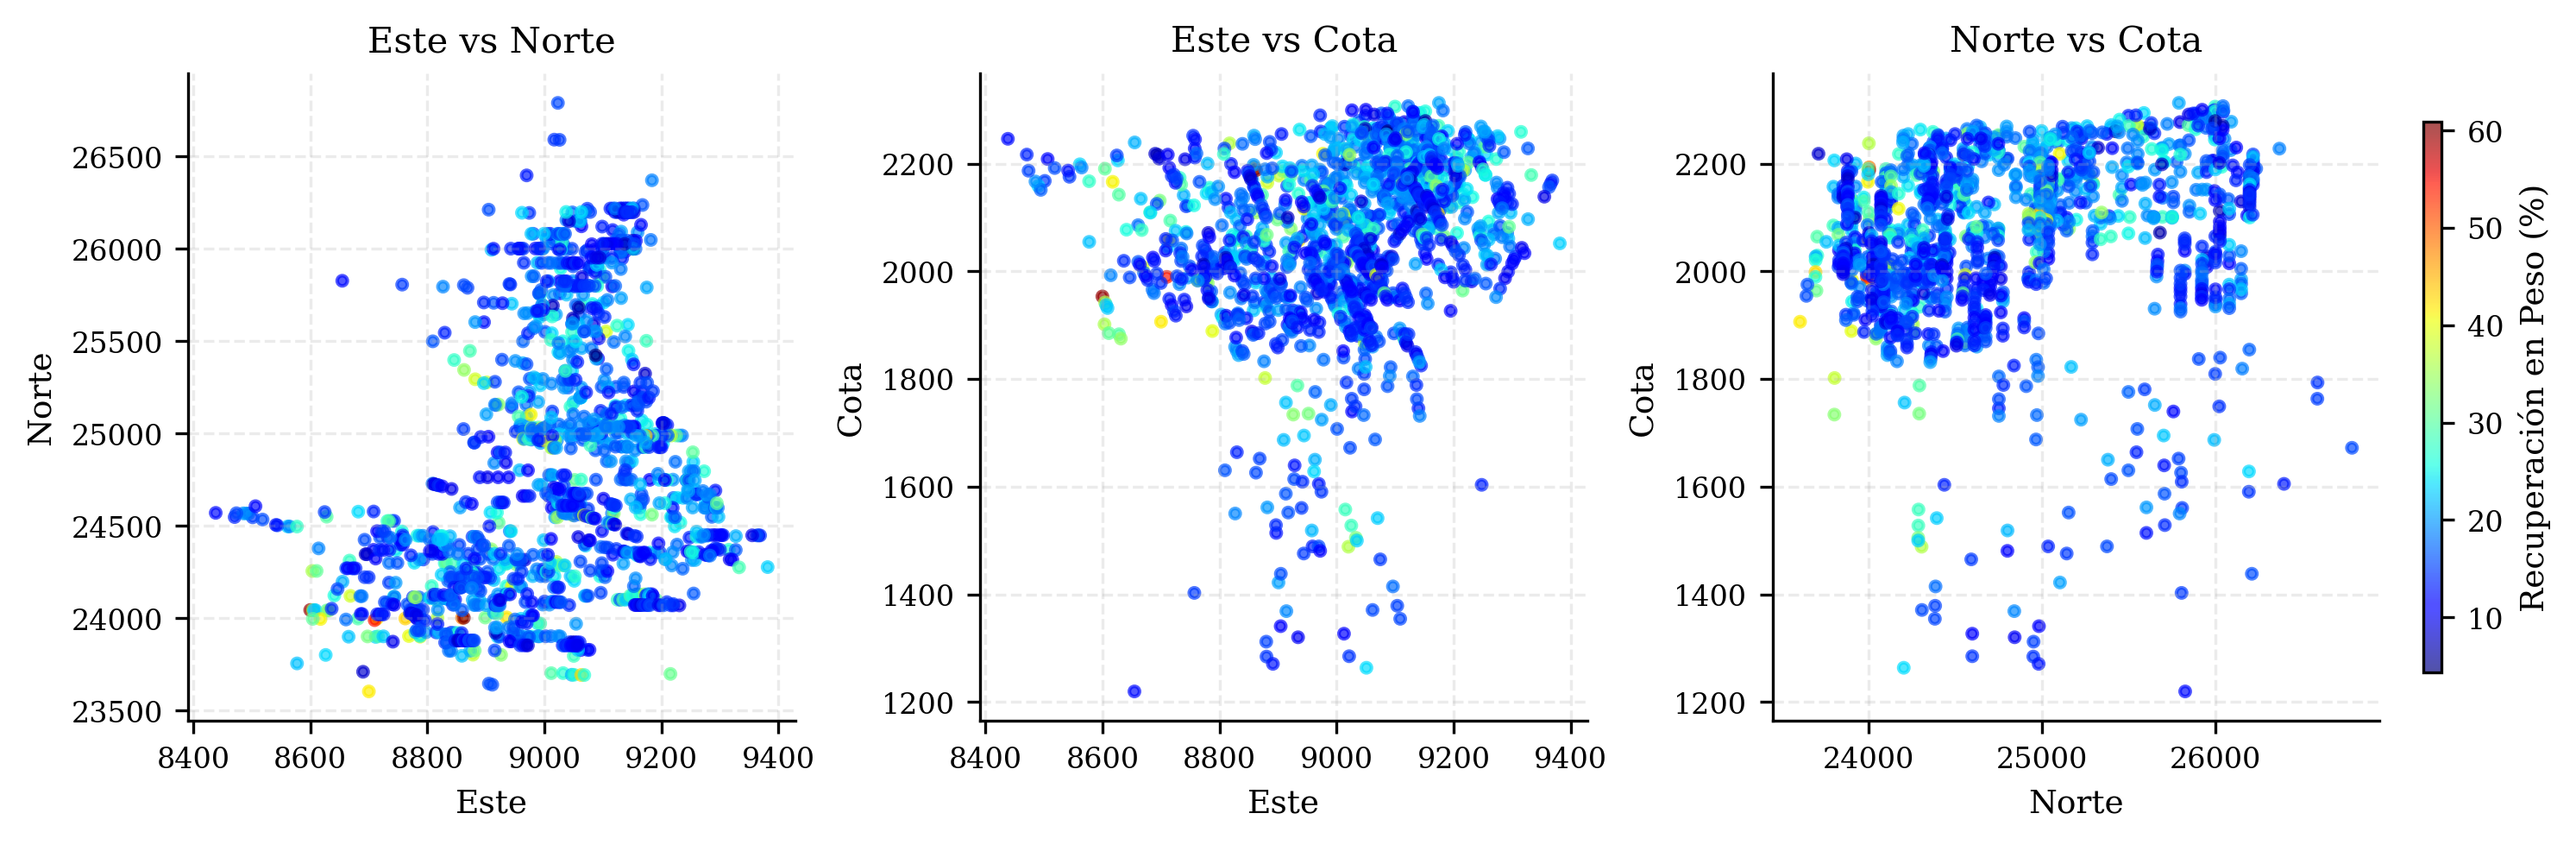
\includegraphics[width=0.9\textwidth]{img_eda/proyecciones_2d_recpe.png}
	\caption{Proyecciones 2D de la recuperación en peso en los planos Este-Norte, 
		Este-Cota y Norte-Cota.}
	\label{fig:2d}
\end{figure}

Finalmente, se analizó la deriva espacial de la variable en las tres direcciones 
principales. La Figura \ref{fig:deriva} muestra que la recuperación en peso no es 
constante a lo largo del yacimiento: en la dirección Norte se observa una caída 
progresiva desde valores cercanos a 28\% en el extremo sur hacia valores de 15\% 
en el norte, mientras que en la dirección Este y Cota las variaciones son más 
moderadas. Esta tendencia confirma que la posición espacial es una variable 
predictora relevante para el modelado.

\begin{figure}[H]
	\centering
	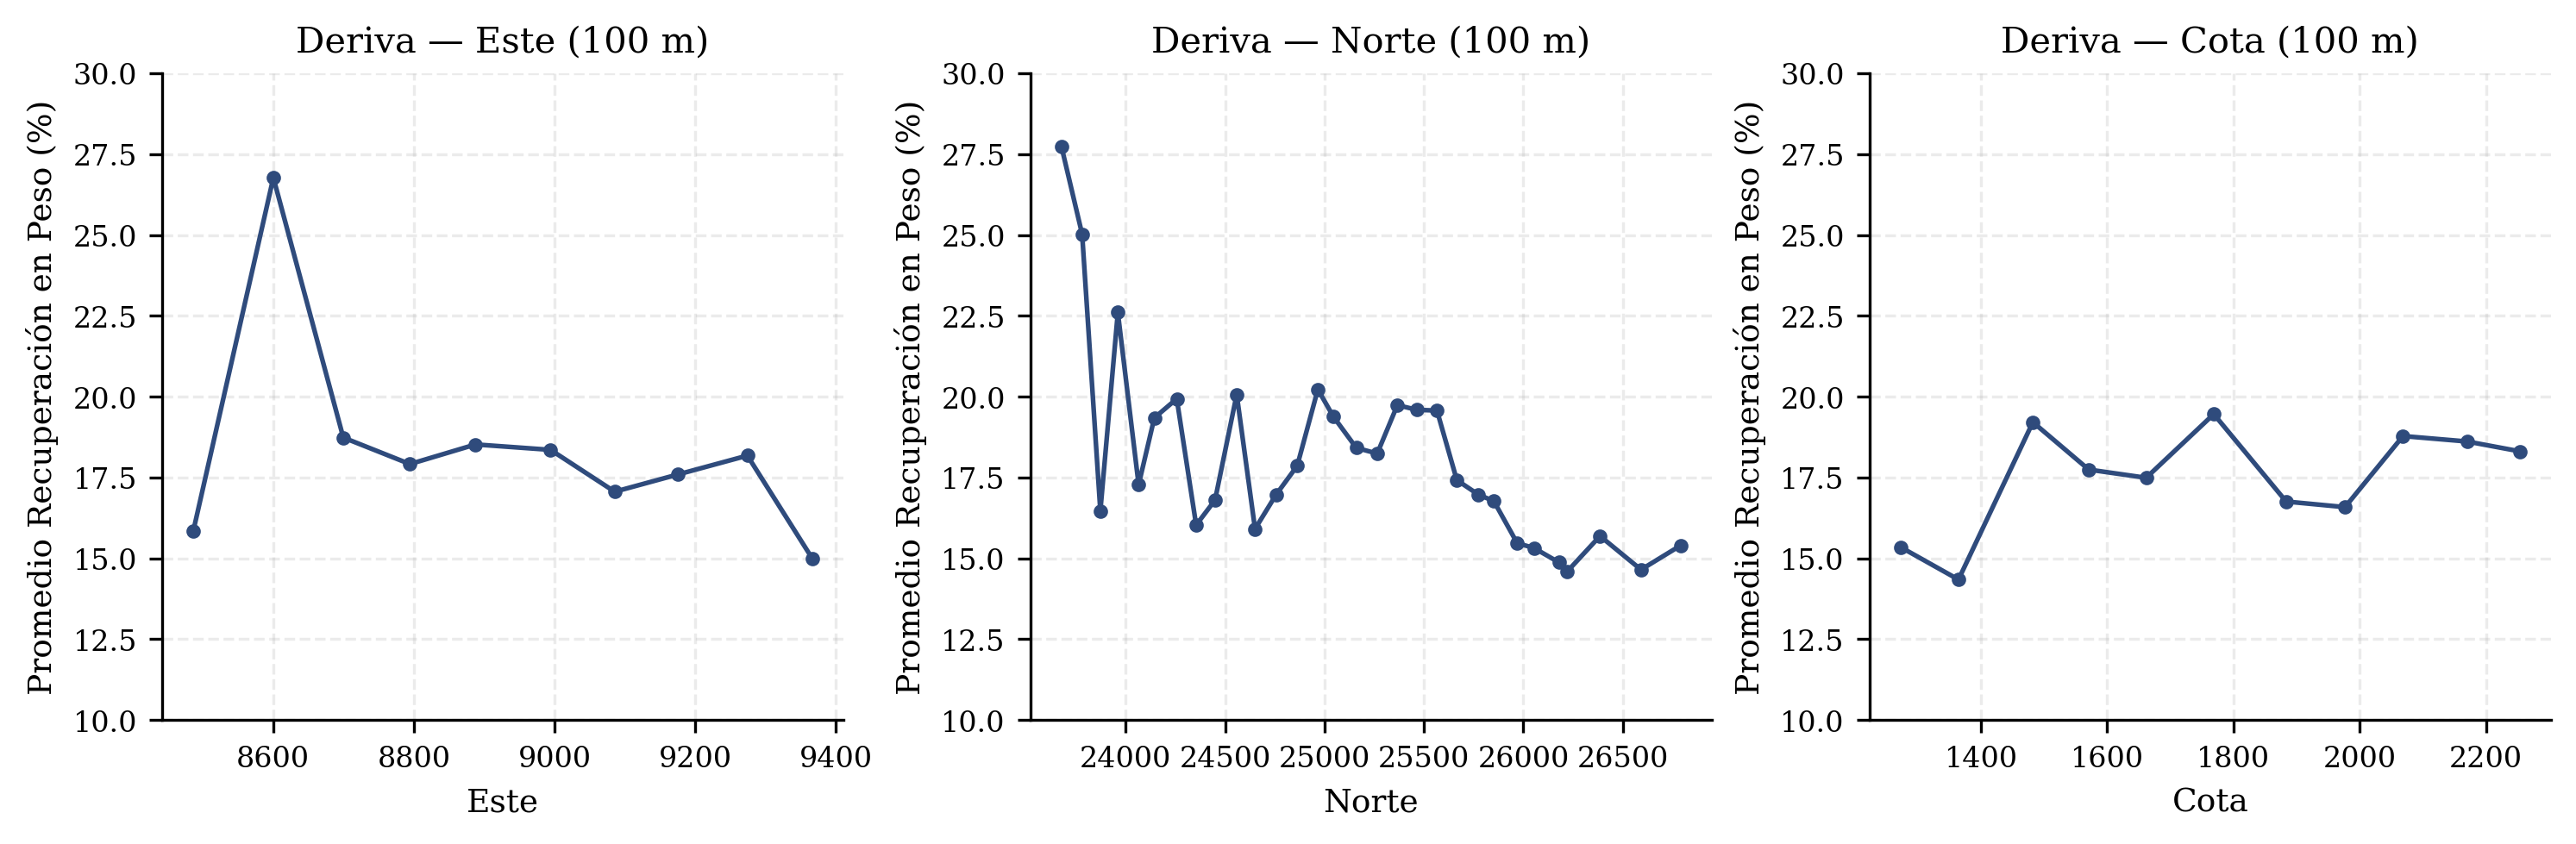
\includegraphics[width=0.9\textwidth]{img_eda/deriva_recpe.png}
	\caption{Deriva espacial de la recuperación en peso en las direcciones 
		Este, Norte y Cota.}
	\label{fig:deriva}
\end{figure}
	

\section{Modelado de datos}

El modelado se estructura en dos etapas. Primero, un análisis de agrupamiento 
no supervisado mediante K-Means, que busca identificar si existen sectores del 
yacimiento con comportamientos metalúrgicos diferenciados. Segundo, el 
entrenamiento de modelos supervisados de Machine Learning para estimar la 
recuperación en peso, cuyos resultados se validan contra el modelo de Kriging 
de la empresa.

Para explorar si el yacimiento presenta zonas con comportamientos metalúrgicos 
distintos, se aplicó el algoritmo K-Means utilizando las coordenadas espaciales 
(Este, Norte y Cota) y la recuperación en peso transformada como variables de 
entrada. El número de clusters se definió en tres, valor que además coincide con 
la segmentación que maneja la empresa en su modelo de bloques, lo que facilita 
la comparación entre ambos enfoques.

La Tabla \ref{tab:kmeans} resume las estadísticas descriptivas de recuperación 
en peso para cada cluster.

\begin{table}[h]
	\centering
	\caption{Estadísticos descriptivos de recuperación en peso por cluster (K-Means).}
	\begin{tabular}{lccccccc}
		\hline
		\textbf{Cluster} & \textbf{N} & \textbf{Promedio} & \textbf{Desv. Est.} & 
		\textbf{Mín.} & \textbf{Mediana} & \textbf{Máx.} \\
		& (1) & (2) & (3) & (4) & (5) & (6) \\
		\hline
		1 & 580 & 18,74 & 5,97 & 6,26  & 17,91 & 42,97 \\
		2 & 371 & 19,56 & 7,94 & 7,22  & 17,73 & 60,87 \\
		3 & 268 & 14,25 & 4,12 & 4,35  & 13,44 & 36,24 \\
		\hline
	\end{tabular}
	\begin{flushleft}
		\small \textit{Nota:} Elaboración propia en base a los datos del estudio.
		(1) = tamaño de muestra, (2) = promedio, (3) = desviación estándar,
		(4) = mínimo valor observado, (5) = mediana, (6) = máximo valor observado.
	\end{flushleft}
	\label{tab:kmeans}
\end{table}

Los clusters 1 y 2 presentan recuperaciones promedio similares, cercanas al 19\%, 
aunque el cluster 2 muestra mayor dispersión y contiene los valores más altos del 
yacimiento. El cluster 3 se diferencia claramente con una recuperación promedio 
de 14,25\% y menor variabilidad. La Figura \ref{fig:kmeans_3d} muestra que esta 
separación también tiene coherencia espacial, con los tres grupos ocupando 
sectores distintos del yacimiento.

\begin{figure}[H]
	\centering
	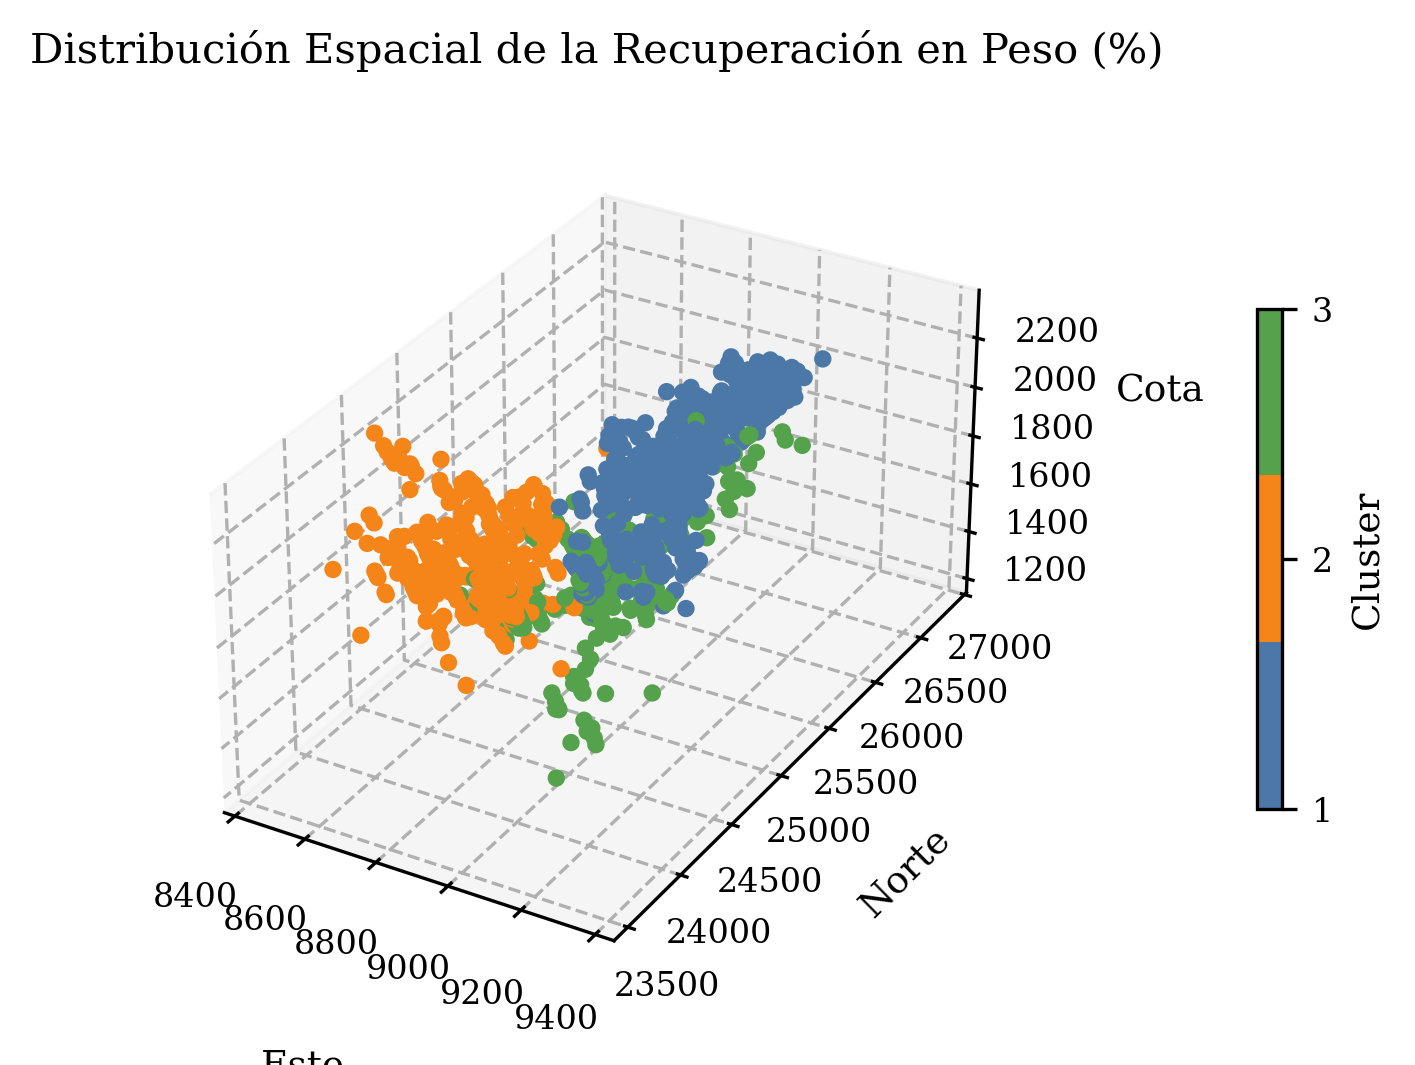
\includegraphics[width=0.8\textwidth]{img_modelado/kmeans_clusters_3d.png}
	\caption{Visualización 3D de los clusters definidos por K-Means.}
	\label{fig:kmeans_3d}
\end{figure}

\begin{figure}[H]
	\centering
	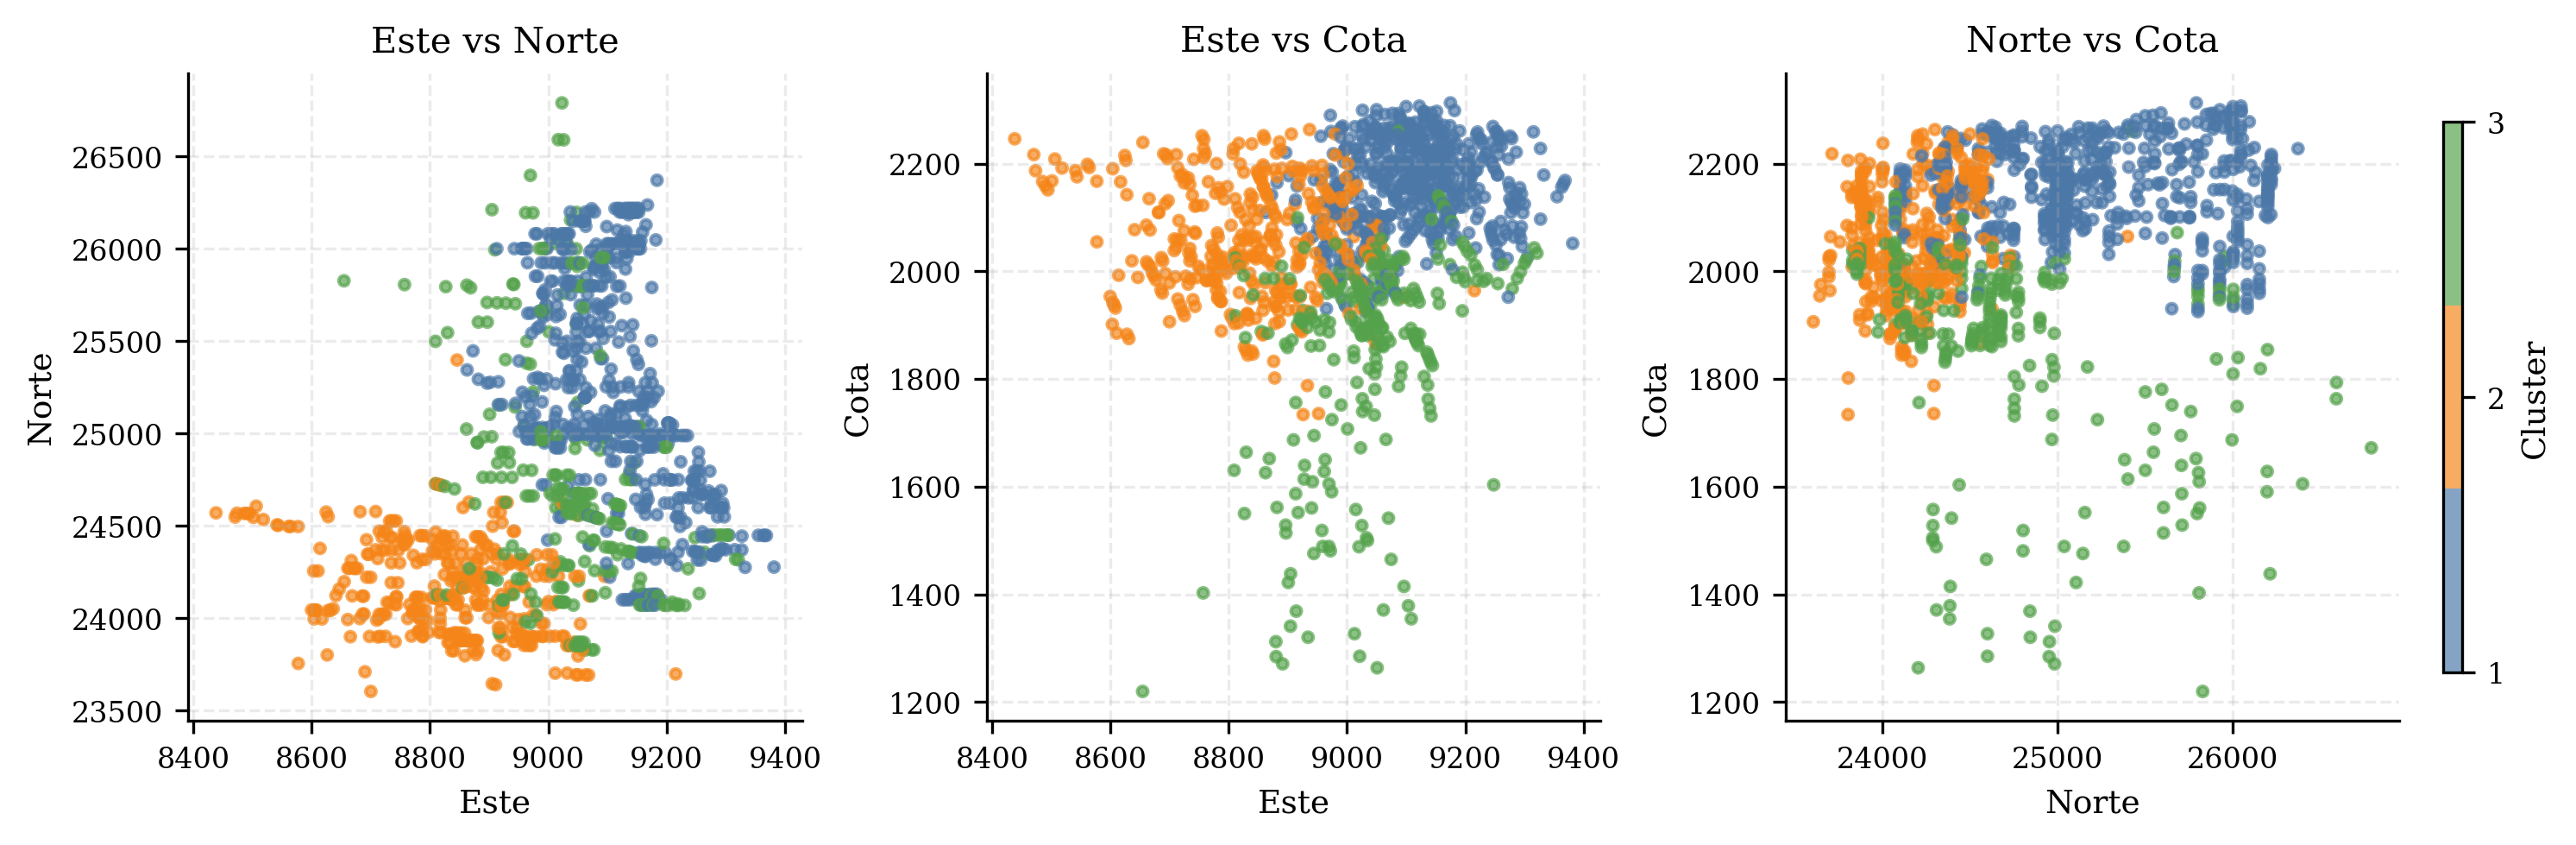
\includegraphics[width=0.9\textwidth]{img_modelado/kmeans_clusters_proyecciones_2d.png}
	\caption{Proyecciones 2D de los clusters en los planos Este-Norte, 
		Este-Cota y Norte-Cota.}
	\label{fig:kmeans_2d}
\end{figure}

La Figura \ref{fig:kmeans_boxplot} complementa el análisis mostrando la 
distribución de recuperación por cluster y el efecto proporcional, que refleja 
la relación entre la media y la dispersión de cada grupo. El cluster 2 presenta 
el mayor efecto proporcional, lo que indica que en ese sector los valores altos 
de recuperación van acompañados de mayor variabilidad.

\begin{figure}[H]
	\centering
	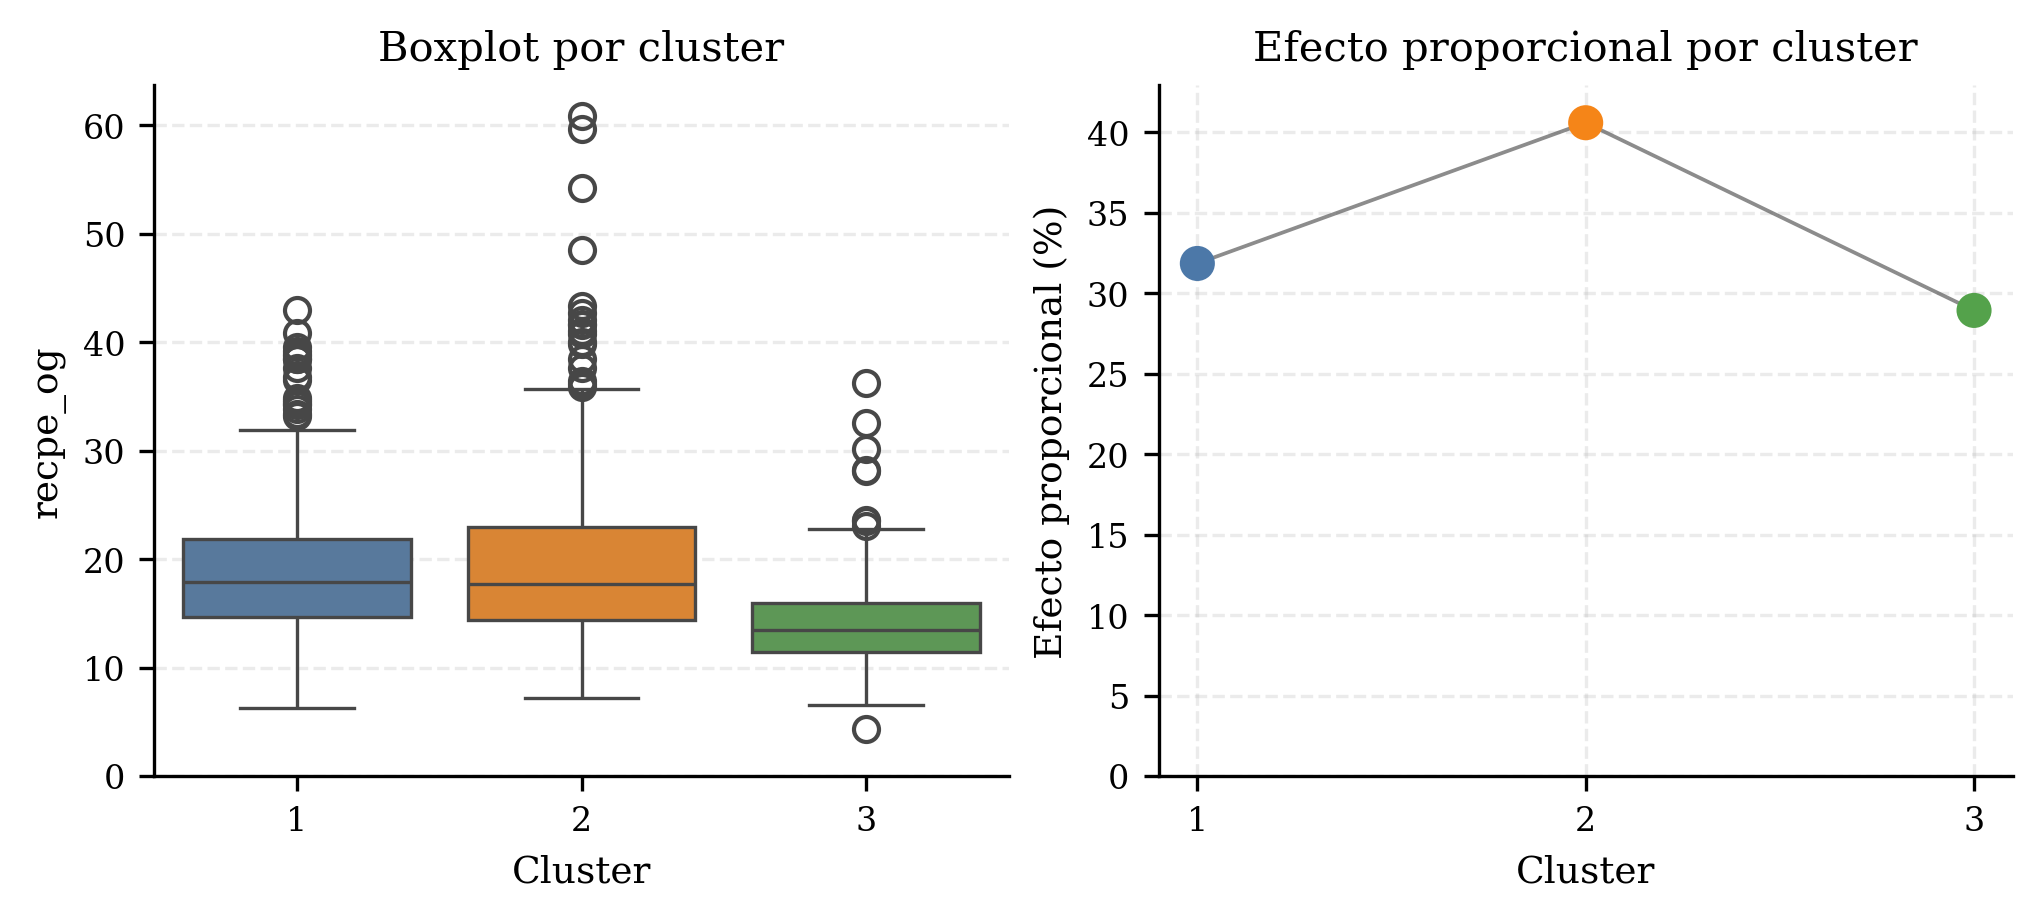
\includegraphics[width=0.9\textwidth]{img_modelado/kmeans_clusters_boxplot_efecto_proporcional.png}
	\caption{Distribución de recuperación en peso por cluster y efecto 
		proporcional.}
	\label{fig:kmeans_boxplot}
\end{figure}

Para la estimación de la recuperación en peso se entrenaron cuatro modelos de 
Machine Learning: K-Nearest Neighbors (KNN), Random Forest, Gradient Boosting y 
XGBoost. Todos los modelos se entrenaron con el 100\% de los 1.219 datos 
disponibles, utilizando las coordenadas espaciales (Este, Norte y Cota) como 
variables predictoras. La validación se realizó de forma externa, comparando las 
predicciones de cada modelo contra los valores reales en los 1.219 puntos del 
emparejamiento descrito en la sección 2.5, usando el Kriging de la empresa como 
referencia bajo las mismas condiciones.

La Tabla \ref{tab:resultados} resume las métricas de desempeño de todos los modelos.

\begin{table}[h]
	\centering
	\caption{Métricas de desempeño de los modelos de estimación.}
	\begin{tabular}{lcccc}
		\hline
		\textbf{Modelo} & \textbf{N} & \textbf{$R^2$} & \textbf{RMSE} & \textbf{MAPE} \\
		& (1) & (2) & (3) & (4) \\
		\hline
		Kriging (empresa)  & 1.219 & 0,796 & 2,992 & 10,5\% \\
		KNN                & 1.219 & 0,630 & 4,032 & 13,3\% \\
		Gradient Boosting  & 1.219 & 0,387 & 5,187 & 19,6\% \\
		XGBoost            & 1.219 & 0,364 & 5,282 & 20,0\% \\
		Random Forest      & 1.219 & 0,342 & 5,372 & 20,3\% \\
		\hline
	\end{tabular}
	\begin{flushleft}
		\small \textit{Nota:} Elaboración propia en base a los datos del estudio.
		(1) = tamaño de muestra, (2) = coeficiente de determinación, 
		(3) = raíz del error cuadrático medio, (4) = error porcentual absoluto medio.
	\end{flushleft}
	\label{tab:resultados}
\end{table}

El Kriging de la empresa obtiene el mejor desempeño con un $R^2$ de 0,796 y un 
MAPE de 10,5\%. Entre los modelos de Machine Learning, KNN es el que mejor 
resultado alcanza con un $R^2$ de 0,630 y un MAPE de 13,3\%, mientras que los 
modelos basados en árboles de decisión quedan considerablemente por debajo. Las 
Figuras \ref{fig:knn}, \ref{fig:gb}, \ref{fig:xgb} y \ref{fig:rf} muestran los 
gráficos de real vs predicho para cada modelo, siempre acompañados del resultado 
del Kriging como referencia.

\begin{figure}[H]
	\centering
	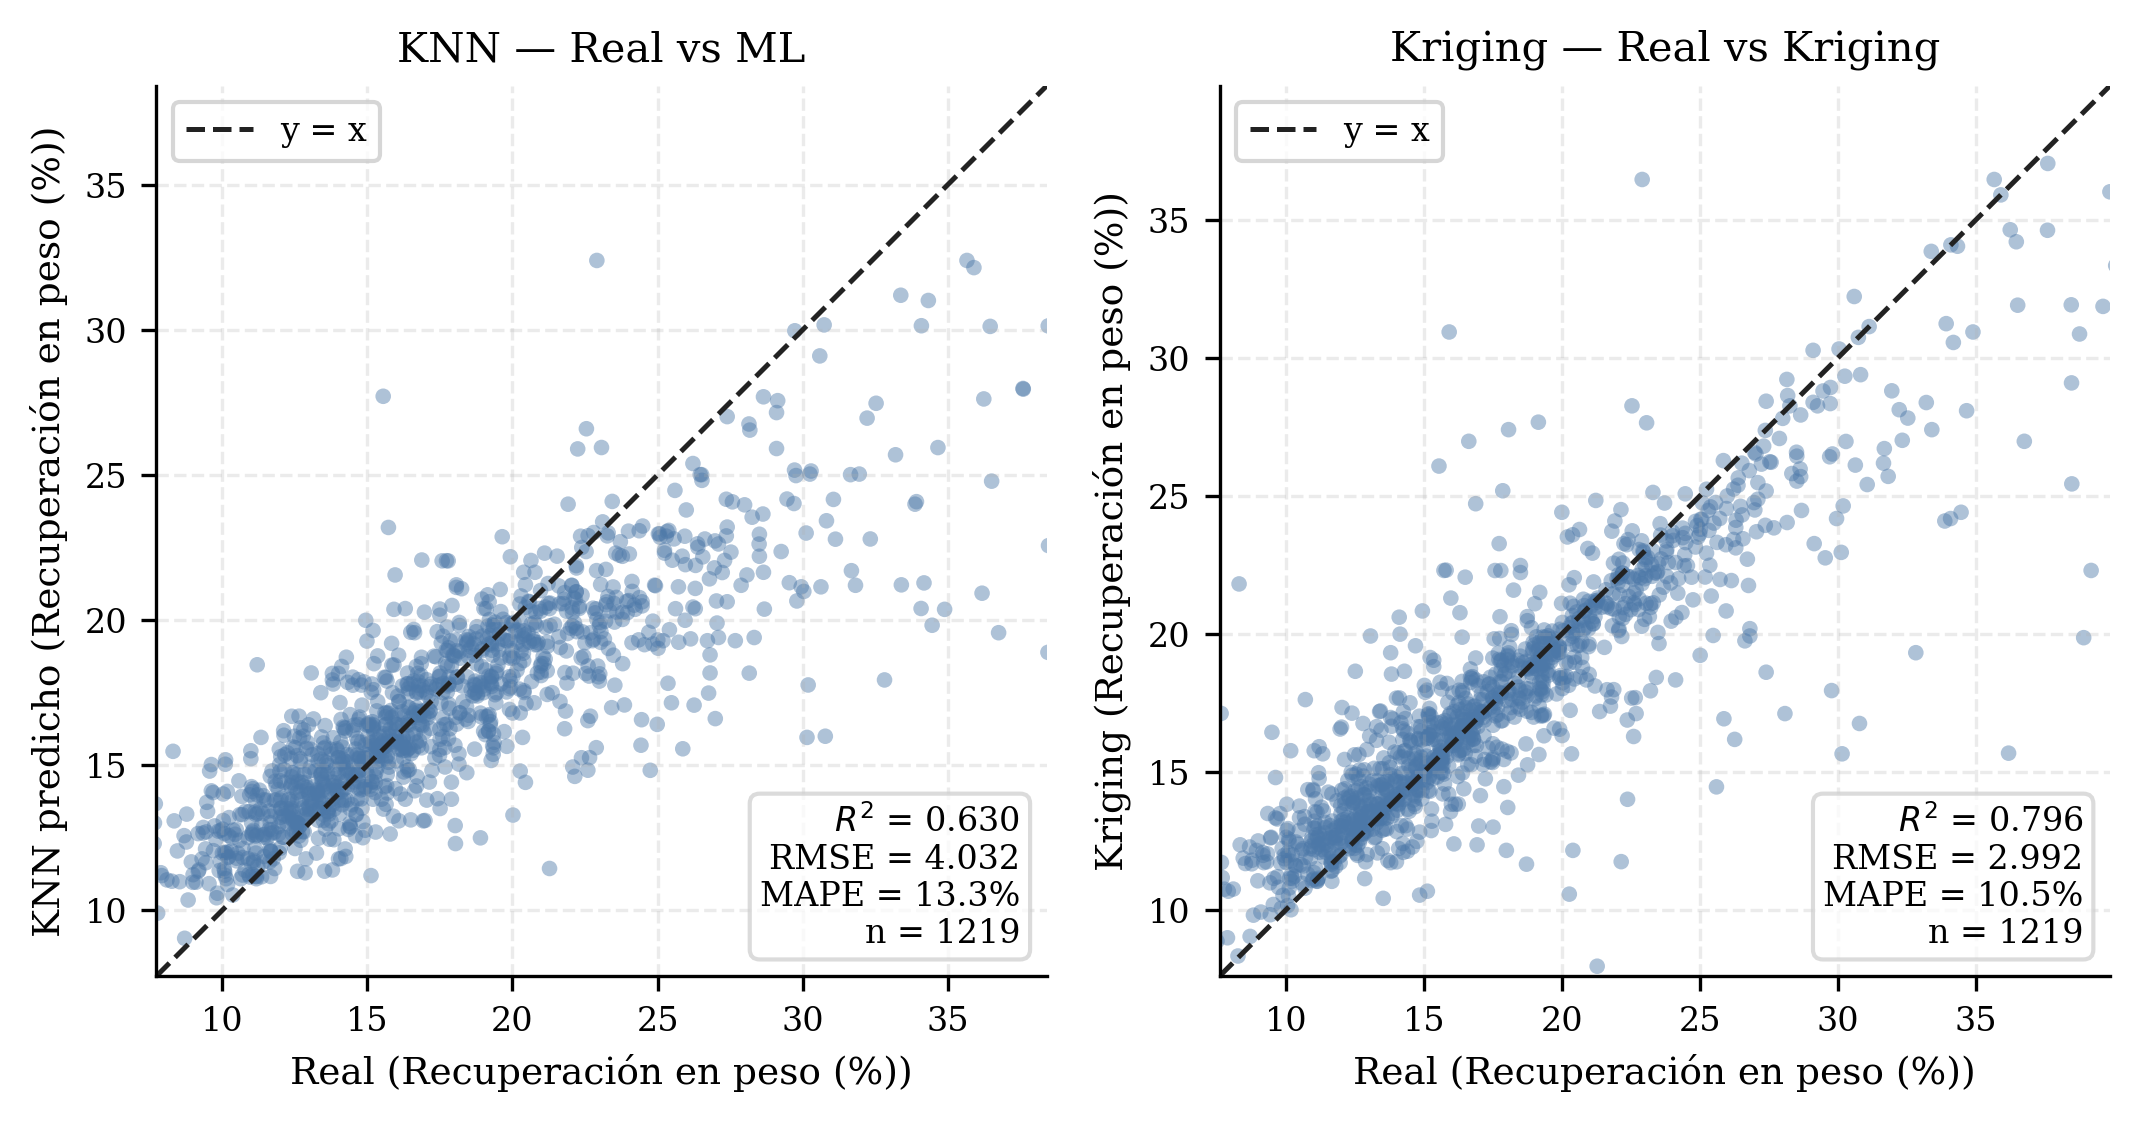
\includegraphics[width=0.9\textwidth]{img_modelado/knn_vs_kriging.png}
	\caption{Recuperación en peso real vs predicha: KNN y Kriging.}
	\label{fig:knn}
\end{figure}

\begin{figure}[H]
	\centering
	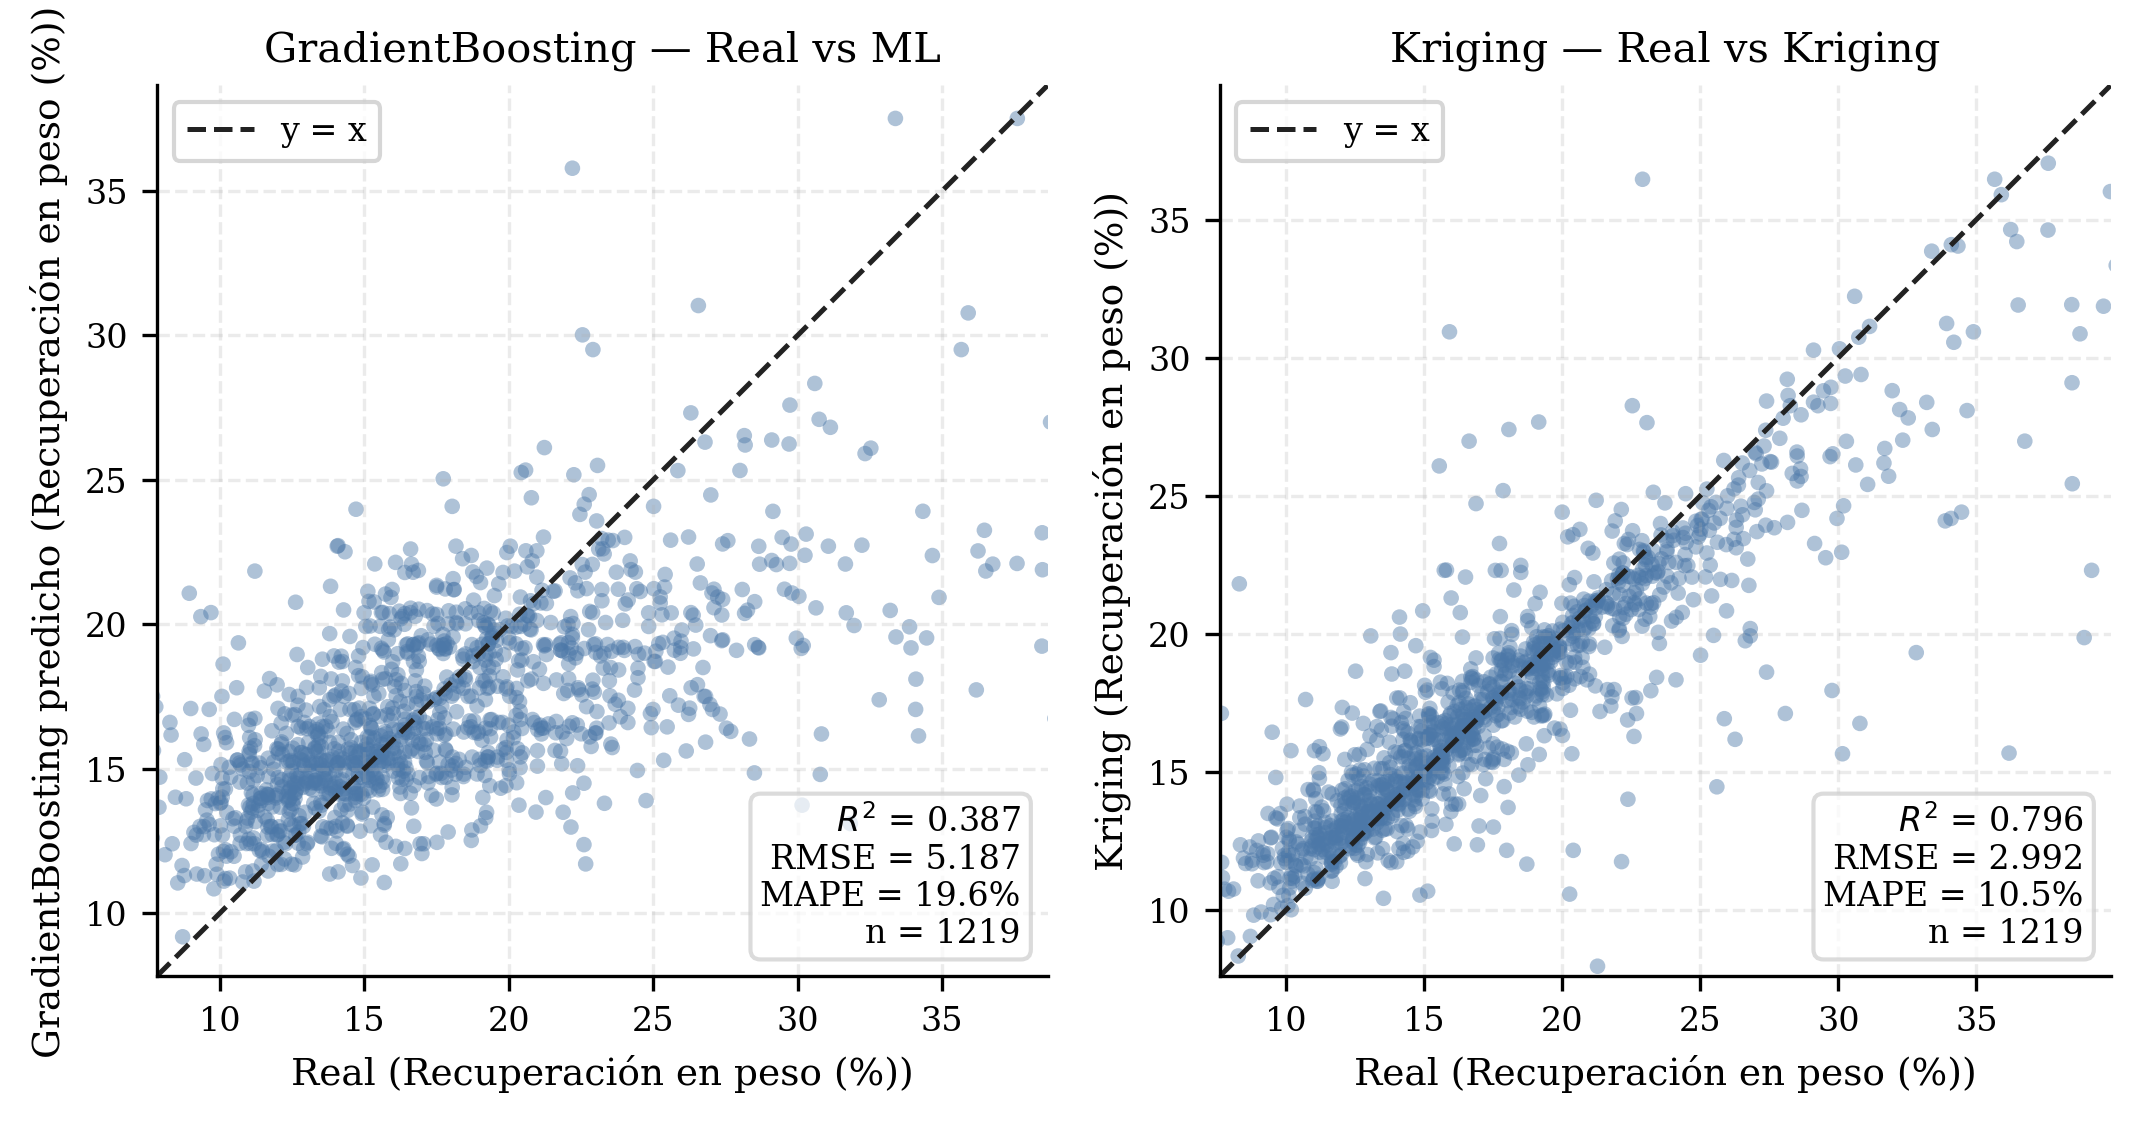
\includegraphics[width=0.9\textwidth]{img_modelado/gradientboosting_vs_kriging.png}
	\caption{Recuperación en peso real vs predicha: Gradient Boosting y Kriging.}
	\label{fig:gb}
\end{figure}

\begin{figure}[H]
	\centering
	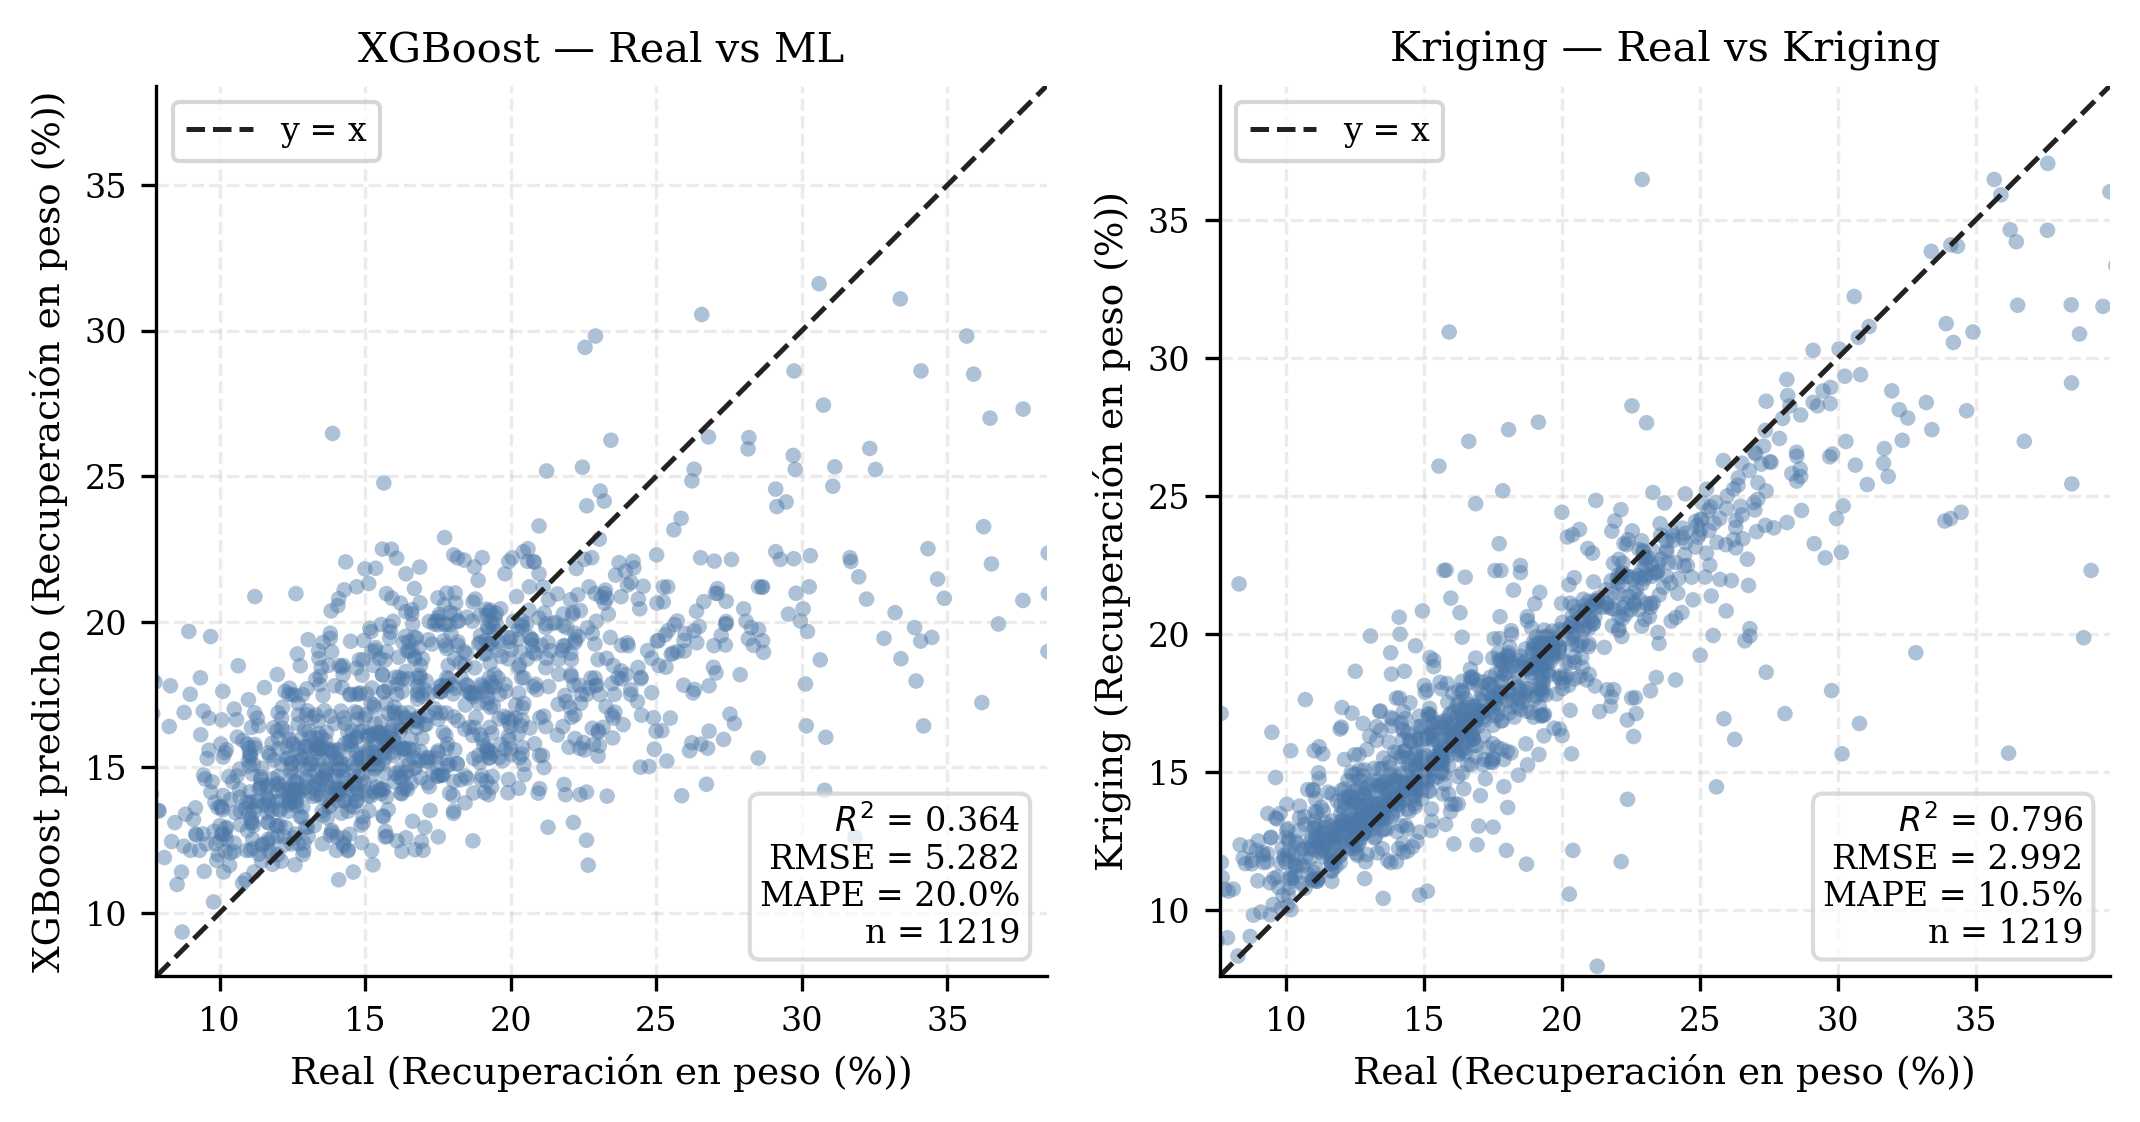
\includegraphics[width=0.9\textwidth]{img_modelado/xgboost_vs_kriging.png}
	\caption{Recuperación en peso real vs predicha: XGBoost y Kriging.}
	\label{fig:xgb}
\end{figure}

\begin{figure}[H]
	\centering
	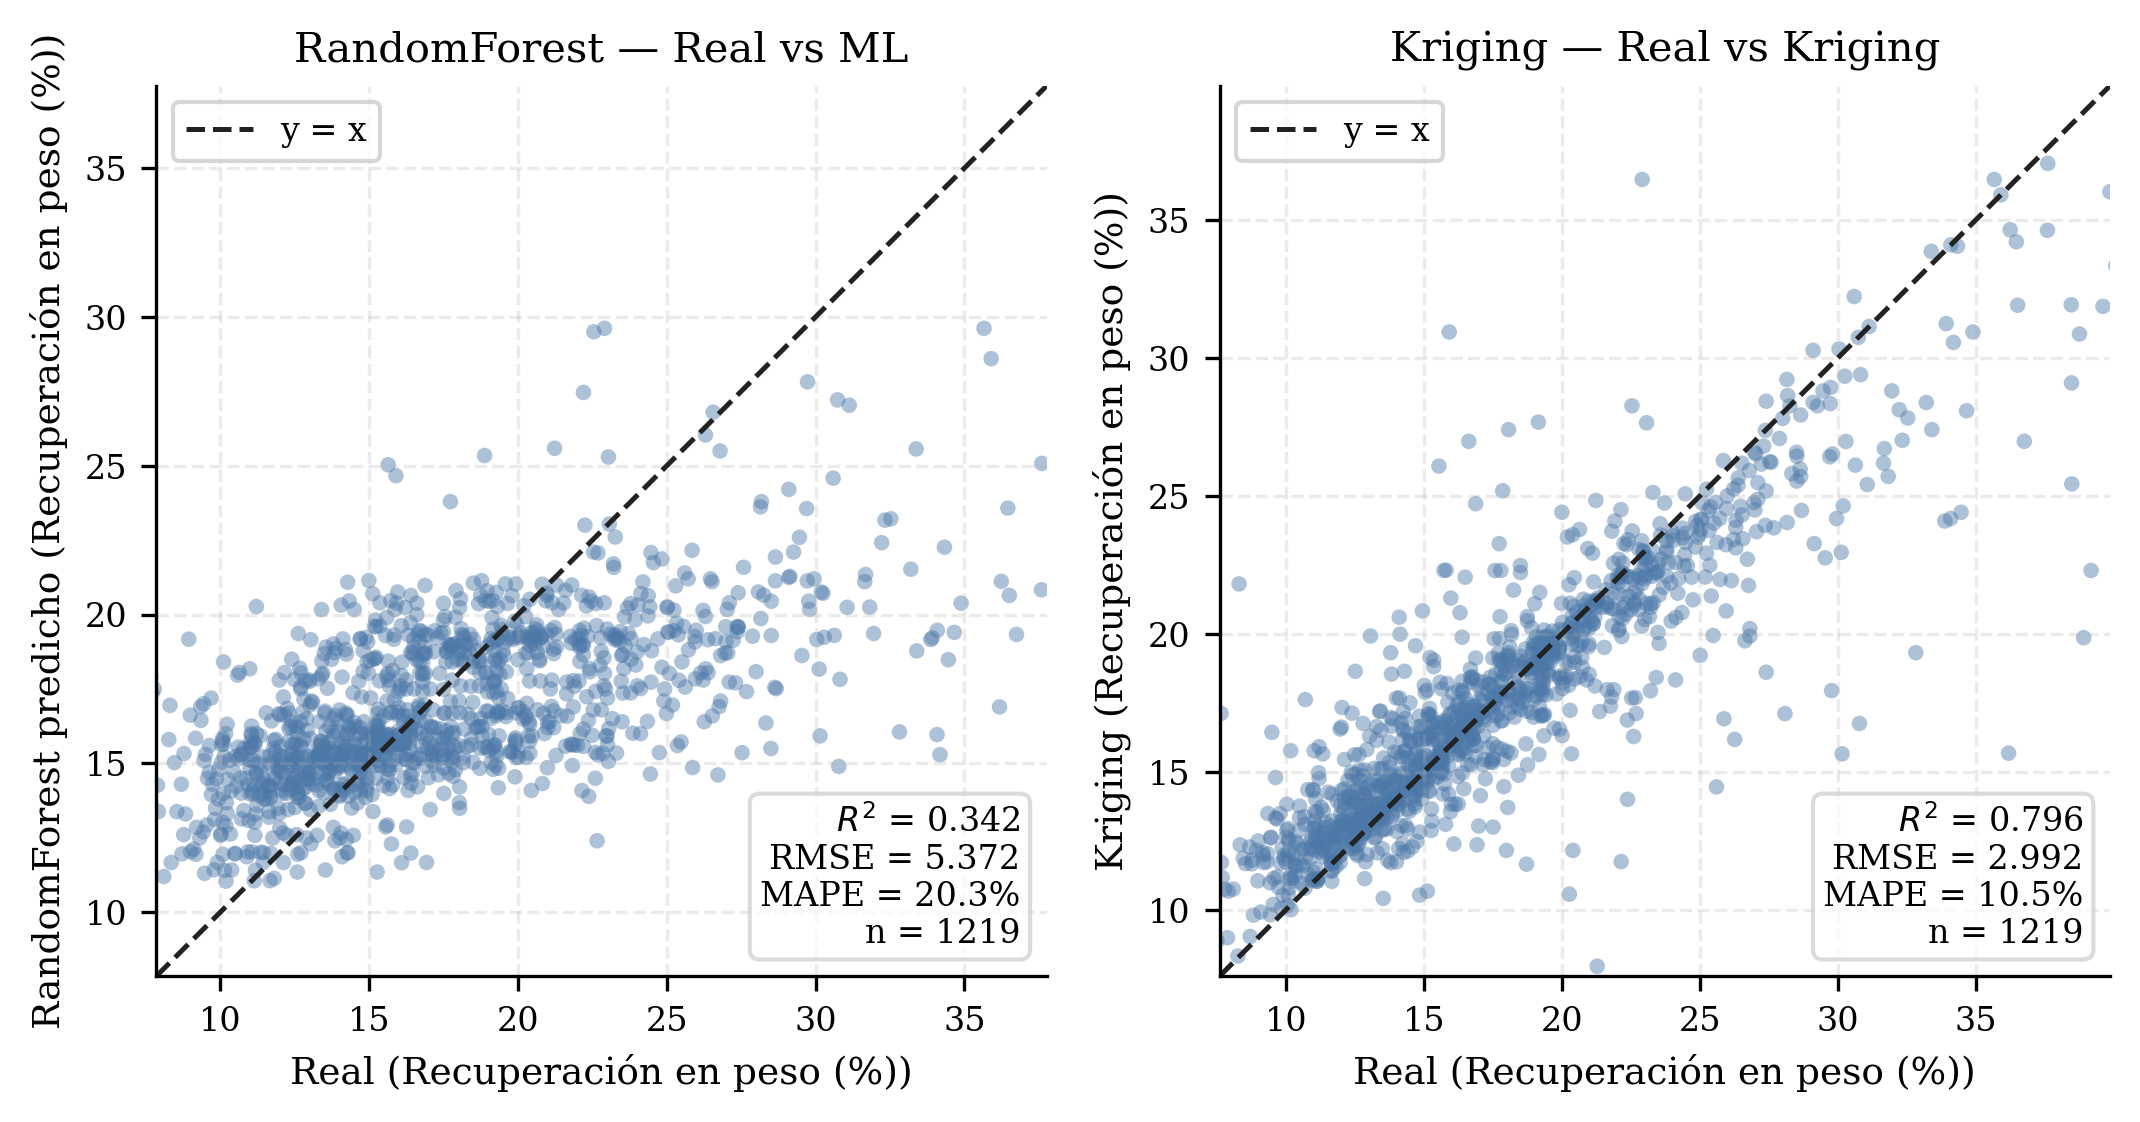
\includegraphics[width=0.9\textwidth]{img_modelado/randomforest_vs_kriging.png}
	\caption{Recuperación en peso real vs predicha: Random Forest y Kriging.}
	\label{fig:rf}
\end{figure}


Para complementar la evaluación, se analizó si los modelos logran respetar el 
comportamiento espacial de los datos originales. La Figura 
\ref{fig:histogramas} compara las distribuciones de recuperación en peso 
estimadas por cada modelo contra la distribución original y la del Kriging. 
Se observa que KNN es el modelo que mejor reproduce la forma general de la 
distribución, mientras que los modelos basados en árboles tienden a concentrar 
sus predicciones en un rango más estrecho, perdiendo representatividad en los 
extremos.

\begin{figure}[H]
	\centering
	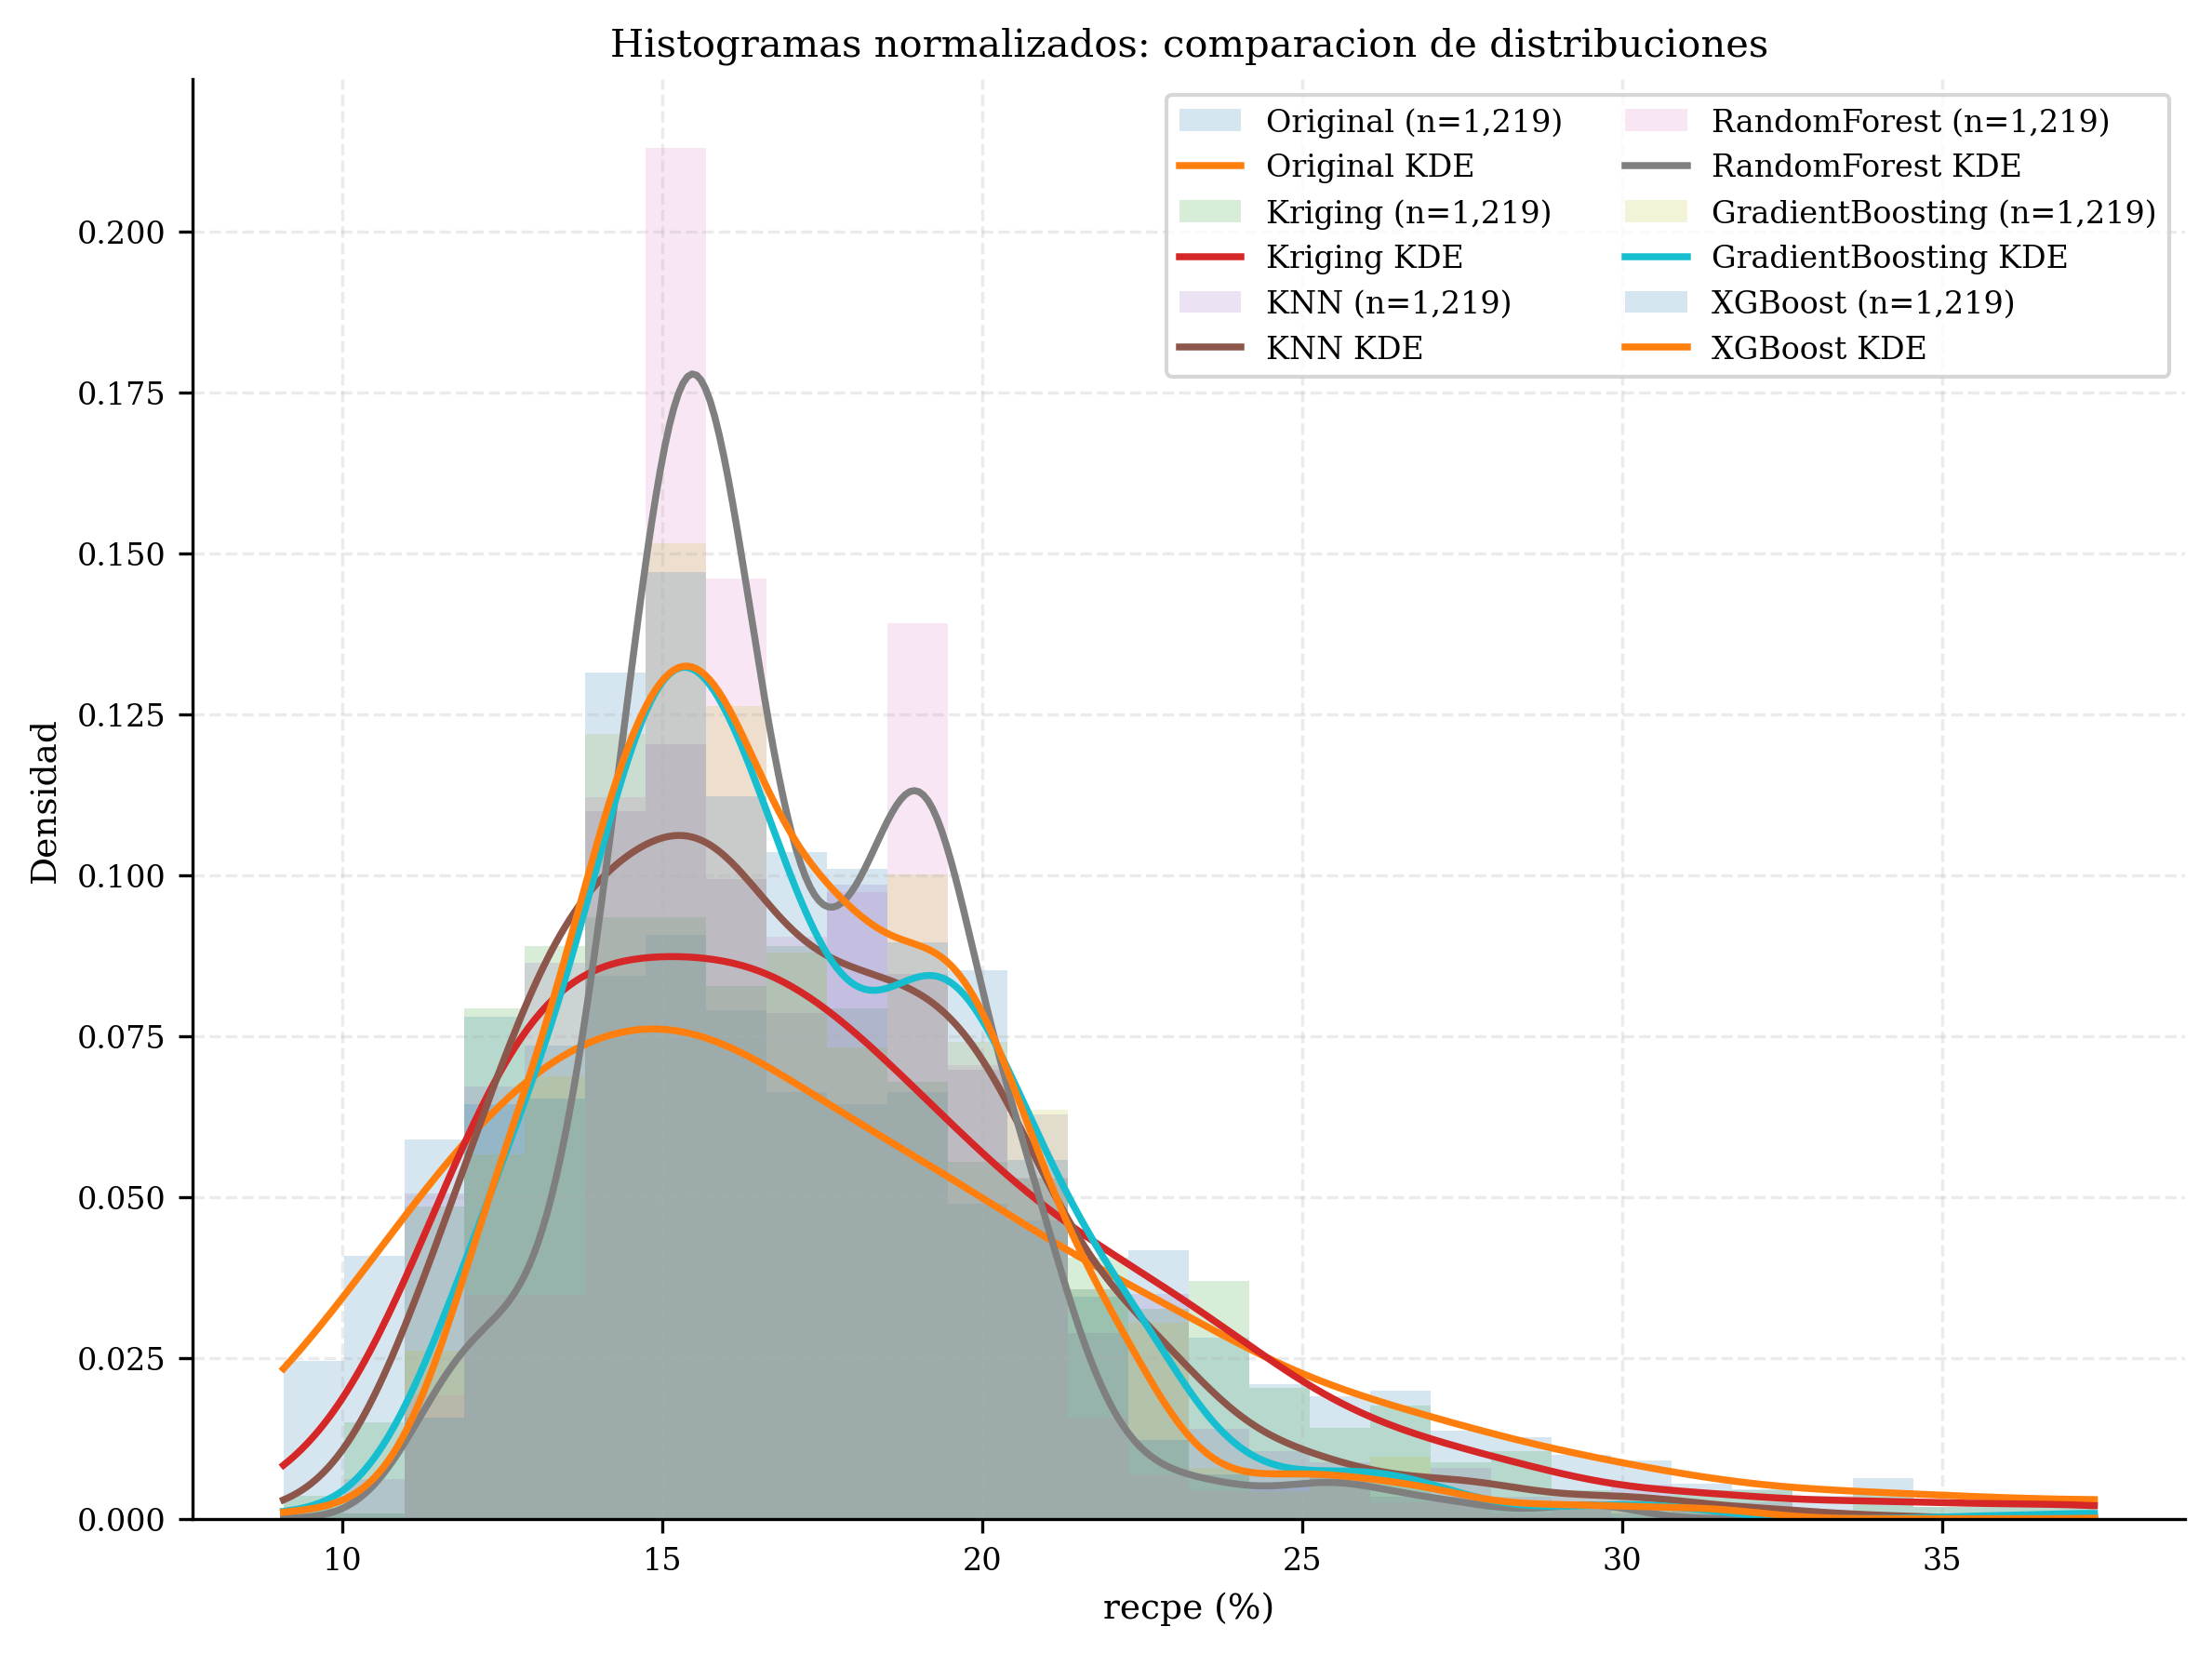
\includegraphics[width=0.9\textwidth]{img_modelado/histogramas_normalizados.png}
	\caption{Comparación de distribuciones de recuperación en peso: datos 
		originales, Kriging y modelos de Machine Learning.}
	\label{fig:histogramas}
\end{figure}

Las Figuras \ref{fig:deriva_este}, \ref{fig:deriva_norte} y \ref{fig:deriva_cota} 
muestran la deriva espacial de las estimaciones en las tres direcciones principales. 
En general, todos los modelos logran seguir la tendencia global de los datos 
originales, aunque con distintos niveles de ajuste. KNN y Kriging son los que más se aproximan a la curva original en las tres direcciones, mientras que los modelos basados en árboles presentan mayor suavizado y pierden algunas variaciones locales, especialmente en la 
dirección Este.

\begin{figure}[H]
	\centering
	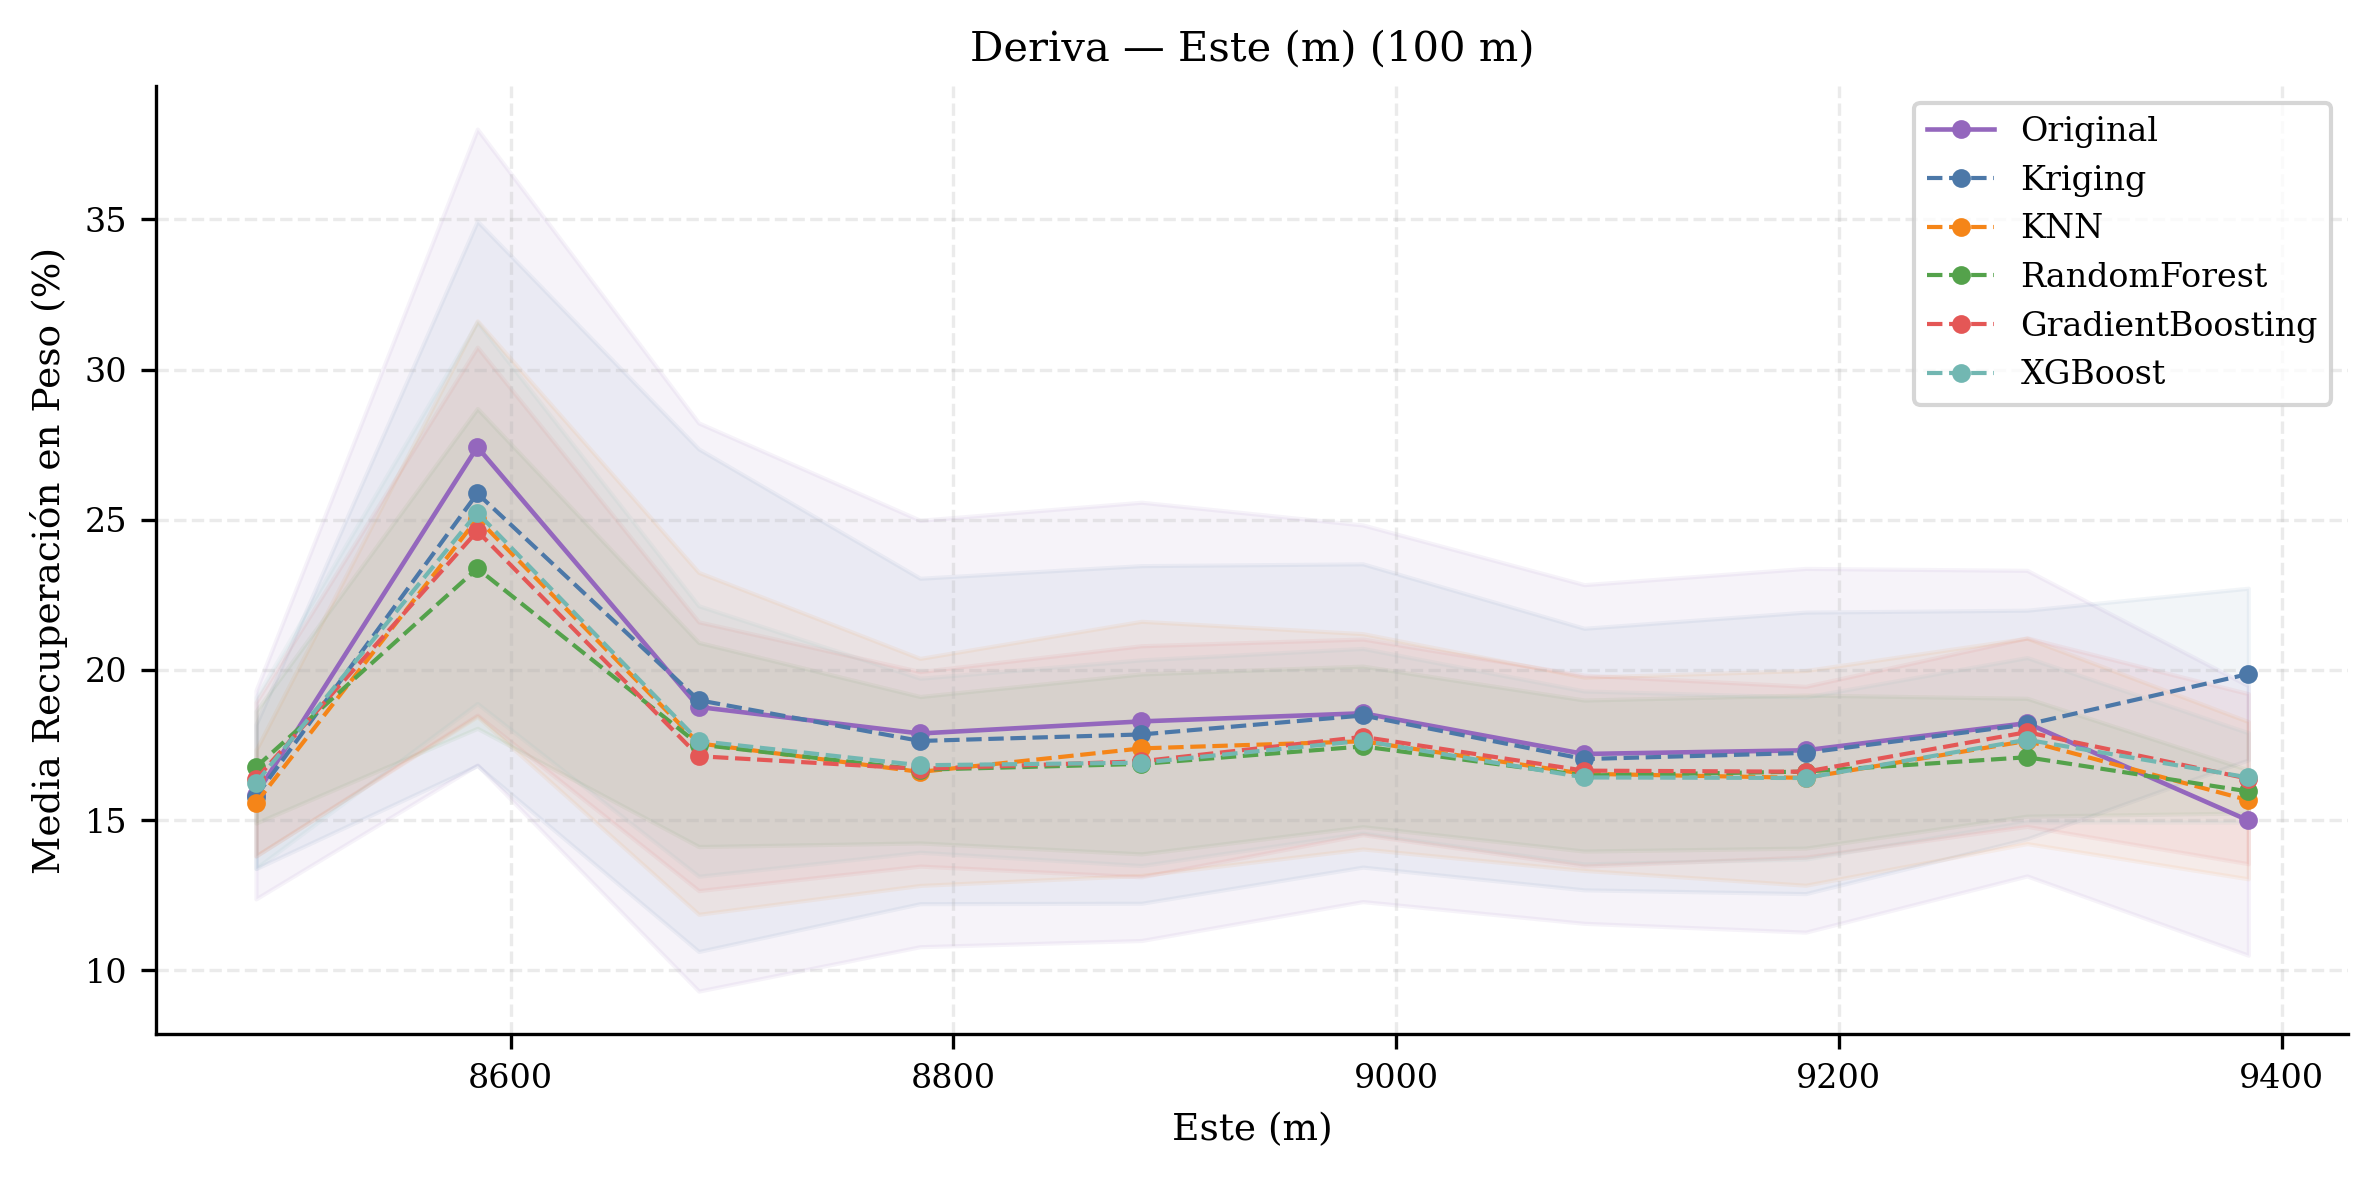
\includegraphics[width=0.9\textwidth]{img_modelado/deriva_este.png}
	\caption{Deriva espacial en la dirección Este: comparación entre datos 
		originales, Kriging y modelos de Machine Learning.}
	\label{fig:deriva_este}
\end{figure}

\begin{figure}[H]
	\centering
	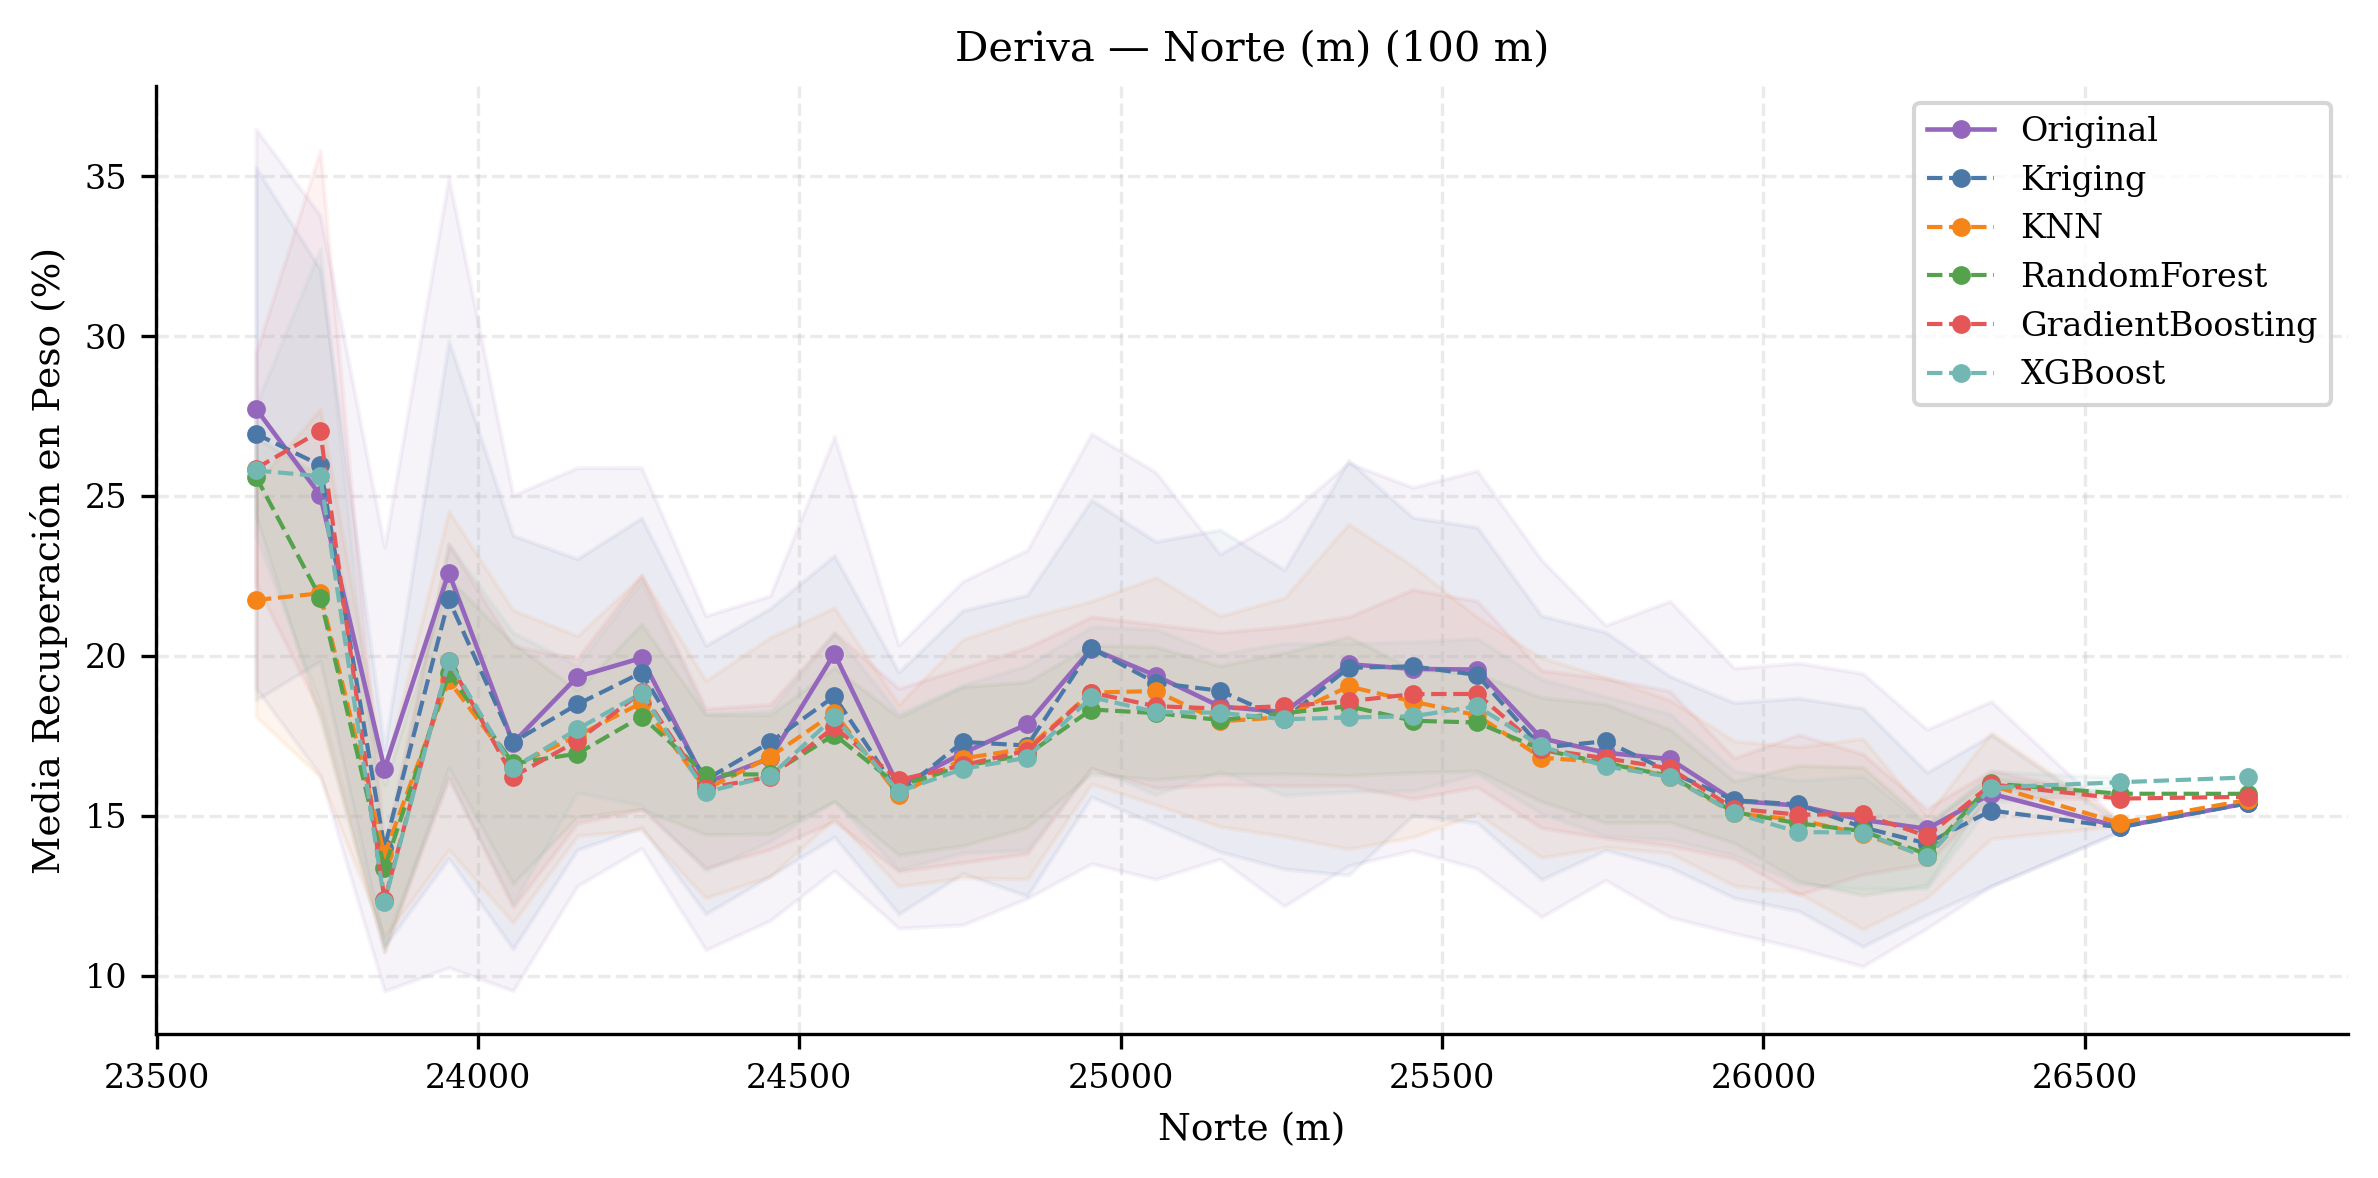
\includegraphics[width=0.9\textwidth]{img_modelado/deriva_norte.png}
	\caption{Deriva espacial en la dirección Norte: comparación entre datos 
		originales, Kriging y modelos de Machine Learning.}
	\label{fig:deriva_norte}
\end{figure}

\begin{figure}[H]
	\centering
	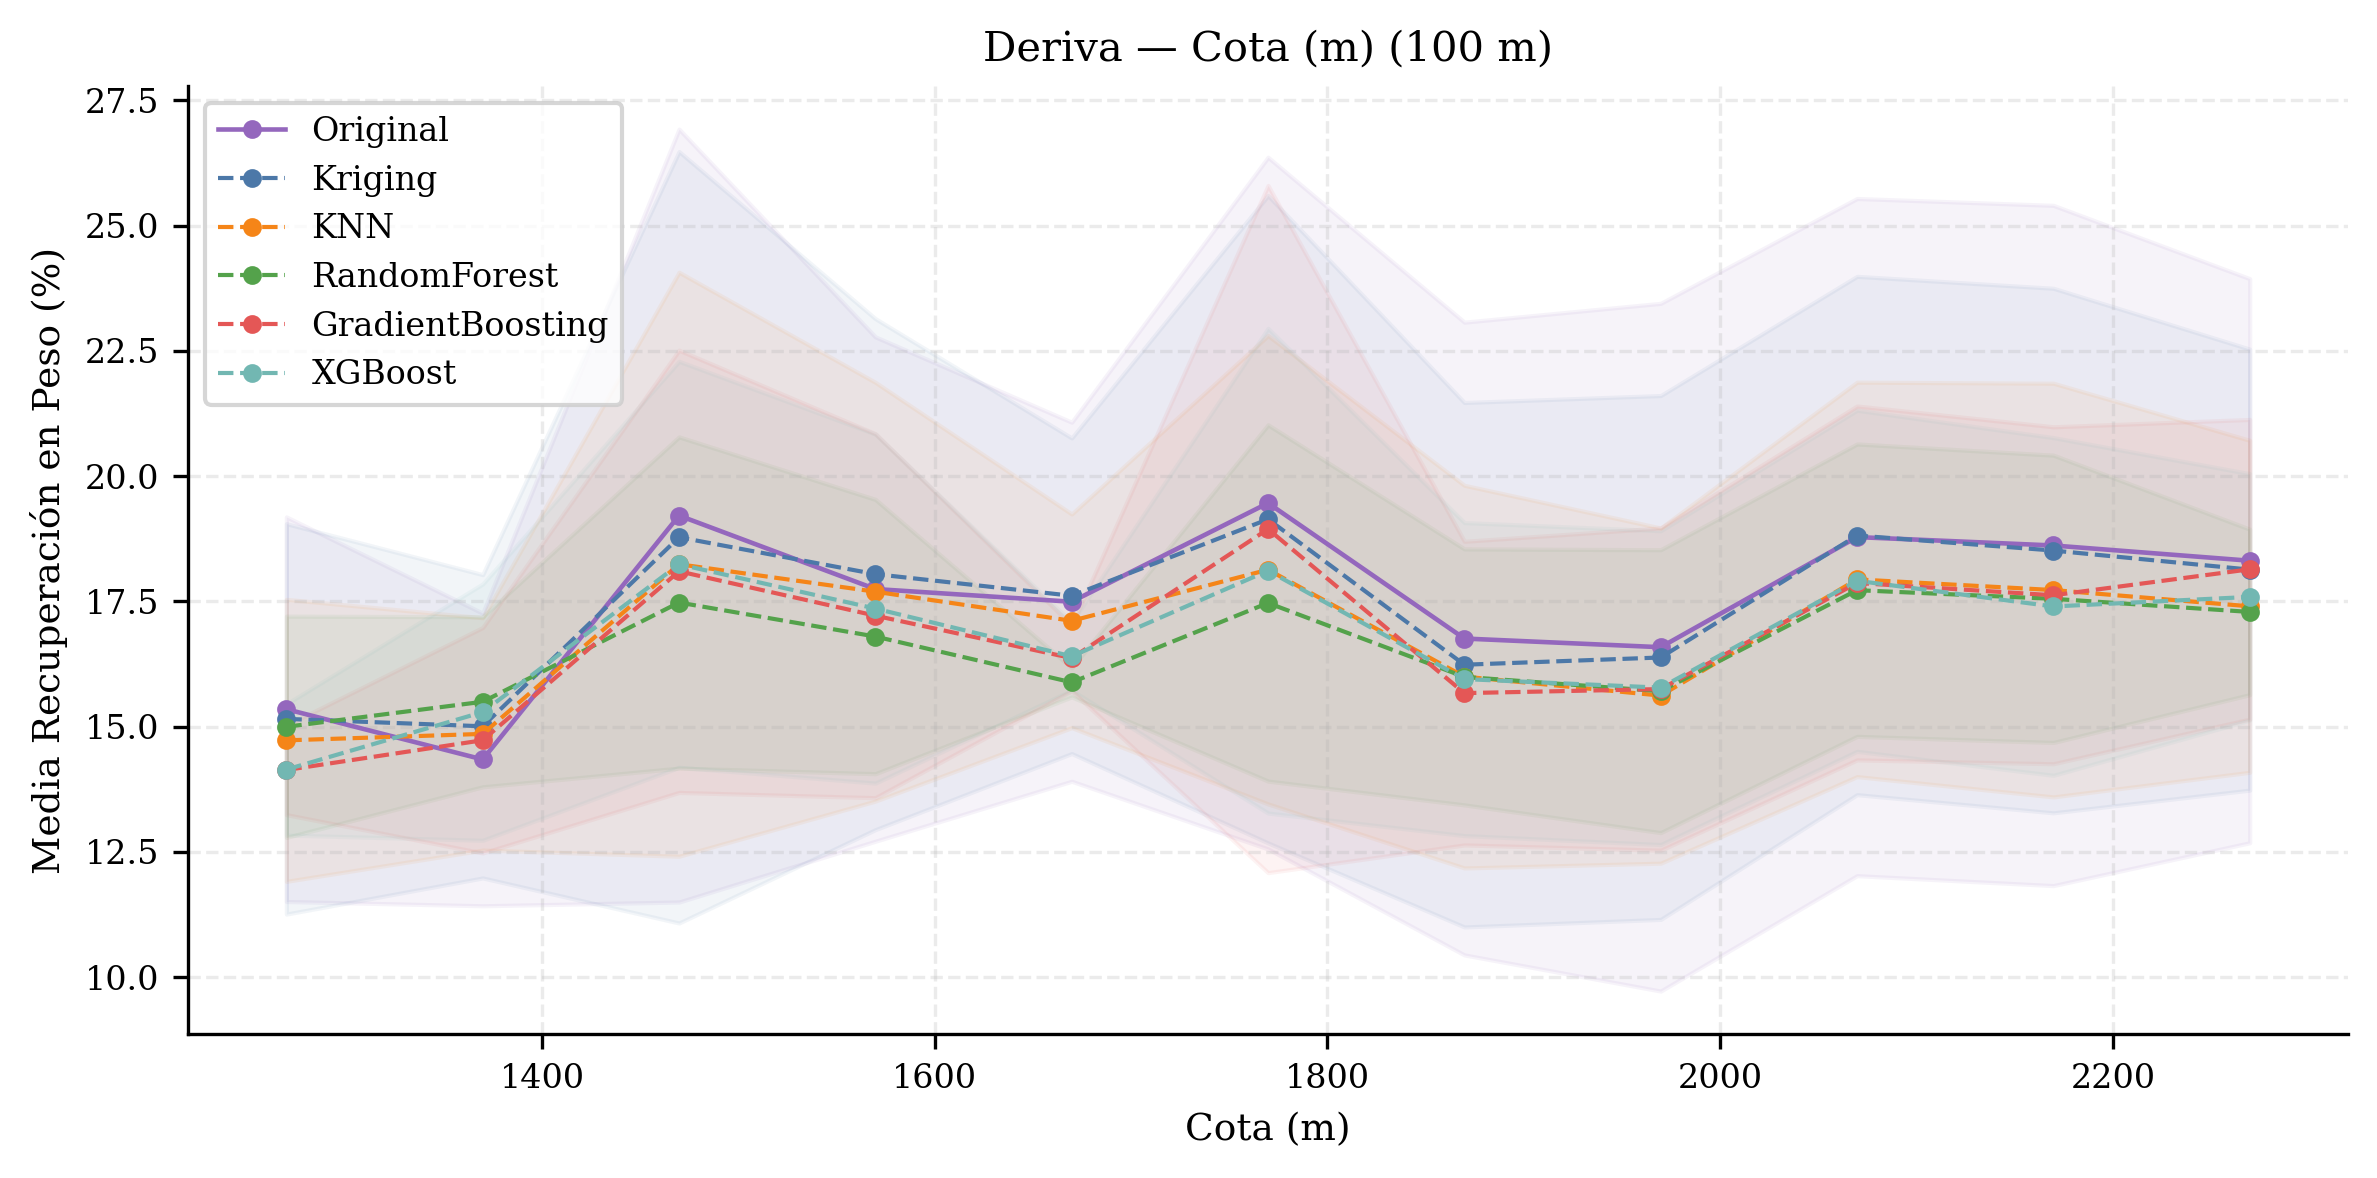
\includegraphics[width=0.9\textwidth]{img_modelado/deriva_cota.png}
	\caption{Deriva espacial en la dirección Cota: comparación entre datos 
		originales, Kriging y modelos de Machine Learning.}
	\label{fig:deriva_cota}
\end{figure}
	
\section{Interpretación de resultados}

Los resultados obtenidos muestran que el Kriging de la empresa sigue siendo el 
método más preciso para estimar la recuperación en peso, con un $R^2$ de 0,796 
y un MAPE de 10,5\%. Entre los modelos de Machine Learning, KNN es el que más 
se acerca con un $R^2$ de 0,630 y un MAPE de 13,3\%, mientras que los modelos 
basados en árboles de decisión, Random Forest, Gradient Boosting y XGBoost, 
quedan todos por debajo de un $R^2$ de 0,39.

El desempeño de KNN tiene una explicación que vale la pena destacar. El modelo 
fue configurado con ponderación por distancia (\textit{weights=``distance''}), 
lo que significa que los vecinos más cercanos tienen mayor influencia en la 
predicción. Dado que los puntos de validación están en promedio a 6,7 metros 
de los puntos de entrenamiento, KNN encuentra vecinos muy similares 
espacialmente, lo que favorece naturalmente su desempeño en este tipo de 
problema. Es importante aclarar que la validación se realizó sobre coordenadas 
distintas a las de entrenamiento, por lo que los resultados obtenidos 
corresponden a una estimación genuinamente externa y no a una memorización de 
los datos de entrenamiento.

El menor desempeño de los modelos basados en árboles se explica por su 
naturaleza algorítmica. Estos modelos aprenden particionando el espacio de 
variables en regiones rectangulares, lo que les dificulta capturar la 
continuidad espacial gradual que caracteriza a un yacimiento. KNN, al basarse 
directamente en distancias entre puntos, es estructuralmente más afín a la 
lógica de la interpolación espacial.

Desde el punto de vista de la coherencia espacial, el análisis de deriva 
mostró que todos los modelos logran reproducir las tendencias generales del 
yacimiento en las tres direcciones, aunque con distintos niveles de ajuste. 
KNN y Kriging son los que mejor siguen la curva original, mientras que los 
modelos de árboles presentan mayor suavizado y pierden algunas variaciones 
locales, especialmente en la dirección Este. En cuanto a la distribución de 
las estimaciones, KNN es también el modelo que mejor reproduce la forma 
general de la distribución original, mientras que los modelos de árboles 
concentran sus predicciones en un rango más estrecho.

En términos prácticos, la brecha de rendimiento entre KNN y el Kriging 
($R^2$ de 0,630 vs 0,796) debe leerse en contexto. El modelo de Kriging fue 
construido por especialistas con experiencia en el yacimiento, ajustando 
manualmente parámetros variográficos y dominios de estimación a lo largo de 
un proceso que puede tomar semanas. El MVP desarrollado en esta tesina, en 
cambio, es un pipeline automatizado que no requiere ese conocimiento experto 
ni software especializado, y que entrega resultados en minutos. Considerando 
esa diferencia en esfuerzo y recursos, un $R^2$ de 0,630 representa un 
resultado aceptable y prometedor para una primera versión del sistema.
	
\section{Conclusión}

	Esta tesina tuvo como objetivo incorporar Machine Learning al flujo de 
	estimación de variables geometalúrgicas, construyendo un MVP en Python que 
	automatice el proceso y permita comparar sus resultados contra el método 
	tradicional utilizado por la empresa. Los resultados muestran que la 
	aproximación es viable, con diferencias de precisión que es importante 
	contextualizar.
	
	Se diseñó un flujo automatizado de preprocesamiento y transformación 
	estadística, se implementó K-Means para la delimitación automática de dominios 
	metalúrgicos espaciales, y se entrenaron y compararon cuatro modelos de 
	aprendizaje supervisado. La validación se realizó de forma externa, 
	contrastando las predicciones de cada modelo contra el modelo de bloques 
	vigente de la empresa sobre los mismos 1.219 puntos de referencia.
	
	El mejor modelo de Machine Learning obtenido, KNN, alcanzó un $R^2$ de 0,630 
	frente al 0,796 del Kriging. Esta diferencia se entiende considerando que el 
	modelo de Kriging fue construido con software propietario de alto costo y un 
	proceso de calibración manual que puede tomar semanas, mientras que el pipeline 
	desarrollado entrega una estimación espacial en minutos, sin requerir ese nivel 
	de recursos ni conocimiento experto especializado.
	
	El espíritu de este trabajo es el de introducir la ciencia de datos en la 
	empresa como herramienta para la estimación de recursos. La ciencia de datos 
	aún no forma parte del flujo de trabajo habitual en esta área, y este MVP 
	busca abrir esa puerta. Existe una oportunidad concreta de ganar velocidad, 
	reducir costos y democratizar el análisis de los propios datos sin depender 
	de software externo.
	
	Como trabajo futuro, incorporar variables geológicas o geometalúrgicas 
	adicionales como predictores, explorar modelos diseñados específicamente para 
	datos espaciales, y aplicar técnicas de validación cruzada que respeten la 
	correlación geográfica de los datos, son pasos naturales para una siguiente 
	versión del MVP. El objetivo de largo plazo es que este tipo de herramientas 
	pueda complementar el flujo de estimación de recursos de la empresa, con el 
	rigor y la transparencia que exige la industria.
	
	\iffalse
	\newpage
	% --- Inicio de Anexos ---
	\appendix
	
	\section{Fundamentos de Geoestadística}
	
	Basado en los apuntes del Prof. Xavier Emery \cite{Emery2007}, se resumen los conceptos fundamentales que sustentan el análisis espacial de esta tesina:
	
	\begin{itemize}
		\item \textbf{Variable Regionalizada:} Es una función numérica $z(x)$ que representa un atributo (como la recuperación en peso) en cada posición $x$ del espacio. Presenta una estructura de continuidad espacial, pero con variaciones irregulares que escapan a representaciones geométricas simples.
		
		\item \textbf{Función Aleatoria:} Se interpreta la variable regionalizada como una realización de una función aleatoria $Z = \{Z(x), x \in D\}$, permitiendo el uso de herramientas probabilísticas para modelar la incertidumbre.
		
		\item \textbf{Hipótesis de Estacionariedad:} Supone que la distribución espacial es invariante ante traslaciones. Esto implica que la esperanza $E[Z(x)] = m$ y la varianza son constantes en el dominio de estudio.
		
		\item \textbf{Variograma:} Es la herramienta central para medir la variabilidad espacial. El variograma teórico se define como:
		\begin{equation}
			\gamma(h) = \frac{1}{2} E[(Z(x) - Z(x+h))^2]
		\end{equation}
		donde $h$ es el vector de separación entre dos puntos. Representa qué tan distintos son los valores a medida que aumenta la distancia.
		
		\item \textbf{Kriging:} Es un método de estimación lineal que busca el valor óptimo en sitios no muestreados, garantizando que el estimador sea insesgado y tenga varianza mínima. Dependiendo del conocimiento de la media ($m$), se distingue entre Kriging Simple (media conocida), Ordinario (media desconocida pero localmente constante) y Universal (presencia de deriva o tendencia espacial).
	\end{itemize}
	
	\section{Modelos de Machine Learning Utilizados}
	
	A continuación, se describen los pilares básicos de los algoritmos implementados en el Producto Mínimo Viable (MVP):
	
	\subsection{K-means (Clustering)}
	Es un algoritmo de aprendizaje no supervisado utilizado para la definición de dominios metalúrgicos. Su objetivo es particionar $n$ observaciones en $k$ clústeres, donde cada observación pertenece al grupo con el centroide ($\mu$) más cercano.
	\begin{itemize}
		\item \textbf{Esencial matemático:} Minimiza la suma de los cuadrados dentro de cada clúster (WCSS):
		\begin{equation}
			J = \sum_{i=1}^{k} \sum_{x \in S_i} ||x - \mu_i||^2
		\end{equation}
	\end{itemize}
	
	\subsection{K-Nearest Neighbors (KNN)}
	Es un método no paramétrico que, para tareas de regresión, estima el valor de una variable basándose en la proximidad de los $k$ vecinos más cercanos en el espacio de características.
	\begin{itemize}
		\item \textbf{Esencial matemático:} La predicción $\hat{y}$ es el promedio simple de los valores de sus vecinos:
		\begin{equation}
			\hat{y} = \frac{1}{k} \sum_{i=1}^{k} y_i
		\end{equation}
	\end{itemize}
	
	\subsection{XGBoost (Extreme Gradient Boosting)}
	Es un algoritmo de ensamble basado en árboles de decisión que utiliza el aumento de gradiente de forma optimizada. Es altamente eficiente para encontrar relaciones no lineales complejas.
	\begin{itemize}
		\item \textbf{Esencial matemático:} Optimiza una función objetivo que equilibra el ajuste a los datos (pérdida $L$) y la complejidad del modelo (regularización $\Omega$):
		\begin{equation}
			Obj(\theta) = \sum_{i} L(y_i, \hat{y}_i) + \sum_{k} \Omega(f_k)
		\end{equation}
		Utiliza expansiones de Taylor para aproximar la pérdida y controlar el sobreajuste mediante penalizaciones en la estructura de los árboles.
	\end{itemize}
	% --- Fin de Anexos ---
	\fi
	
\bibliographystyle{plain}
\bibliography{export}
	
\end{document}